\documentclass[11pt,a4j]{jreport}
\usepackage{enumitem} % リストをカスタマイズするためのパッケージ
\usepackage{comment}
\usepackage{float}
\usepackage{color}
\usepackage{multicol}
\usepackage[dvipdfmx]{pict2e}
\usepackage{wrapfig}
\usepackage{graphicx}
\usepackage{bm}
\usepackage{url}
\usepackage{underscore}
\usepackage{colortbl}
\usepackage{tabularx}
\usepackage{fancyhdr}
\usepackage{ulem}
\usepackage{cite}
\usepackage{amsmath,amssymb,amsfonts}
\usepackage{algorithmic}
\usepackage{textcomp}
\usepackage{xcolor}
\usepackage[ipaex]{pxchfon}
\usepackage[top=30truemm,bottom=30truemm,left=25truemm,right=25truemm]{geometry}

\setlength{\headheight}{15.5pt} % Increase head height
\begin{document}

\thispagestyle{empty}
\begin{center}

\vspace{20mm}
{\Large\noindent 2025年度 卒業(修士)論文}\\
\vspace{40mm}
{\huge\noindent\textbf{AC磁化率測定・NMRによるAu-Al-Tb系}}\\
\medskip
{\huge\noindent\textbf{1/1近似結晶のわけわかめ磁気構造の解明}}\\
\vspace{\baselineskip}
\vspace{40mm}

{\Large\noindent
2025年X月XX日\\
\vspace{\baselineskip}
指導教員 伊藤哲明・小内貴祥 \\
\vspace{\baselineskip}
東京理科大学\\
先進工学研究科物理工学専攻 \\
\vspace{\baselineskip}
8423524 小宮聖智\\
}
\vspace{40mm}

\end{center}

\thispagestyle{empty}
\clearpage

%============================================================================

% 目次の表示
\tableofcontents

%=====================================================================================
\pagestyle{fancy}
\lhead{\rightmark}
\renewcommand{\chaptermark}[1]{\markboth{第\ \normalfont\thechapter\ 章~~#1}{}}
%=====================================================================================

\chapter{はじめに} %章

\section{研究背景} %1.1
準結晶が発見される以前、無機物質の構造は結晶かアモルファス(非結晶)のいずれかであると長い間考えられてきた。しかし、周期構造を持つ結晶やランダムな構造を持つアモルファスとは異なる、特殊な構造を持つ物質群が1980年代初頭に発見され、結晶学の常識を覆した。この特殊な構造は、1984年にダン・シェヒトマンによって発見され、X線回折法により5回回転対称の回折パターンが観測されたことで、その存在が明らかになった。5回回転対称性を持つ単位格子は、従来の結晶学の観点から非常に特殊であり、禁じられた対称性とされていた。通常の結晶は、2次元平面上で三角形や四角形、六角形などのタイルを隙間なく無限に敷き詰めることができ、その結果、単位格子が周期的に並び、物質のどの位置から見ても同じ構造が無限に繰り返される。しかし、5回回転対称の単位格子は、2次元平面上で正五角形を隙間なく敷き詰めることが不可能であるため、無限の周期構造をとることができない。このため、従来の結晶学では5回回転対称性は存在し得ないと考えられていた。ところが、5回回転対称性を持つ物質が実際に発見され、さらに、ロジャー・ペンローズによって考案されたペンローズ・タイリングと呼ばれる5回回転対称性を持つ図形を用いて、周期構造がないにもかかわらず無限に広がる特殊な構造(準周期構造)が実現できることが明らかになった。図\ref{quasicrystalline_structure1}に示すように、ペンローズ・タイリングは2種類の菱形タイルを特定のルールに従って組み合わせることで、非周期的でありながら長距離的な秩序を持つパターンを形成する。このように、準結晶の結晶構造は特殊な準周期構造から成り立っており、その発見は物質科学や数学の分野において新たな研究の道を開いた。また、準結晶は特異な物理的性質を持ち、例えば高い硬度や低い摩擦係数を示すことから、新素材としての応用も期待されている。これらの発見により、結晶学の定義は拡張され、周期的な配置だけでなく、準周期的な配置も結晶として認識されるようになった。準結晶はまた、対称性や秩序の概念に対する我々の理解を深め、自然界や人工構造物における複雑なパターンの研究に貢献している。
\begin{figure}[htbp]
  \centering
  \vspace{4mm}
  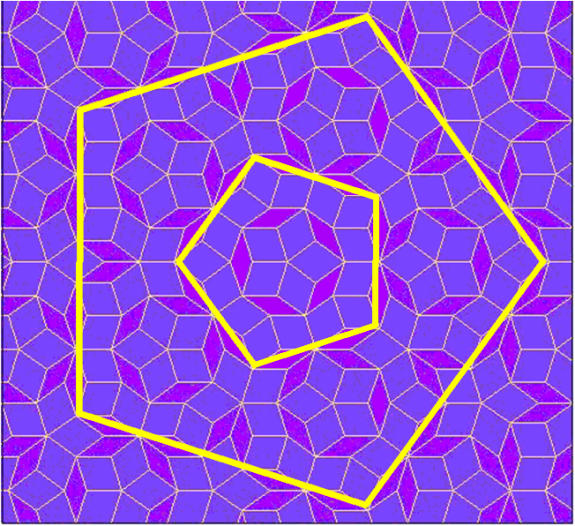
\includegraphics[width=60mm]{./figure/quasicrystalline_structure1.jpg}
  \caption{準結晶の結晶構造}
  \label{quasicrystalline_structure1}
\end{figure}

\section{研究目的}
本研究では、Au-Al-Tb系1/1近似結晶の磁気基底状態の解明を目的としている。図\ref{purpose_of_research}に示すように、通常の結晶は周期的な構造を持つため、スピンが揃いやすく磁気秩序を形成しやすい。一方、アモルファスのようなランダムな構造ではスピン秩序は見られないことが知られている。近年、多くの準結晶が発見され、これらの準結晶の局所構造をもつ近似結晶を用いた研究が進展し、準結晶に関する理解が深まってきた。特に、ランタノイド元素を含む準結晶や近似結晶では、長距離磁気秩序を示す例が報告されているが、準周期構造を持つ準結晶のスピン構造については、いまだに明らかになっていない。そこで本研究では、Au-Al-Tb系1/1近似結晶に対してAC磁化率測定およびAl-NMR測定を行い、マクロ測定とミクロ測定両方の観点から準結晶・近似結晶における磁気基底状態を明らかにすることを目指す。

\begin{figure}[htbp]
  \centering
  \vspace{10mm}
  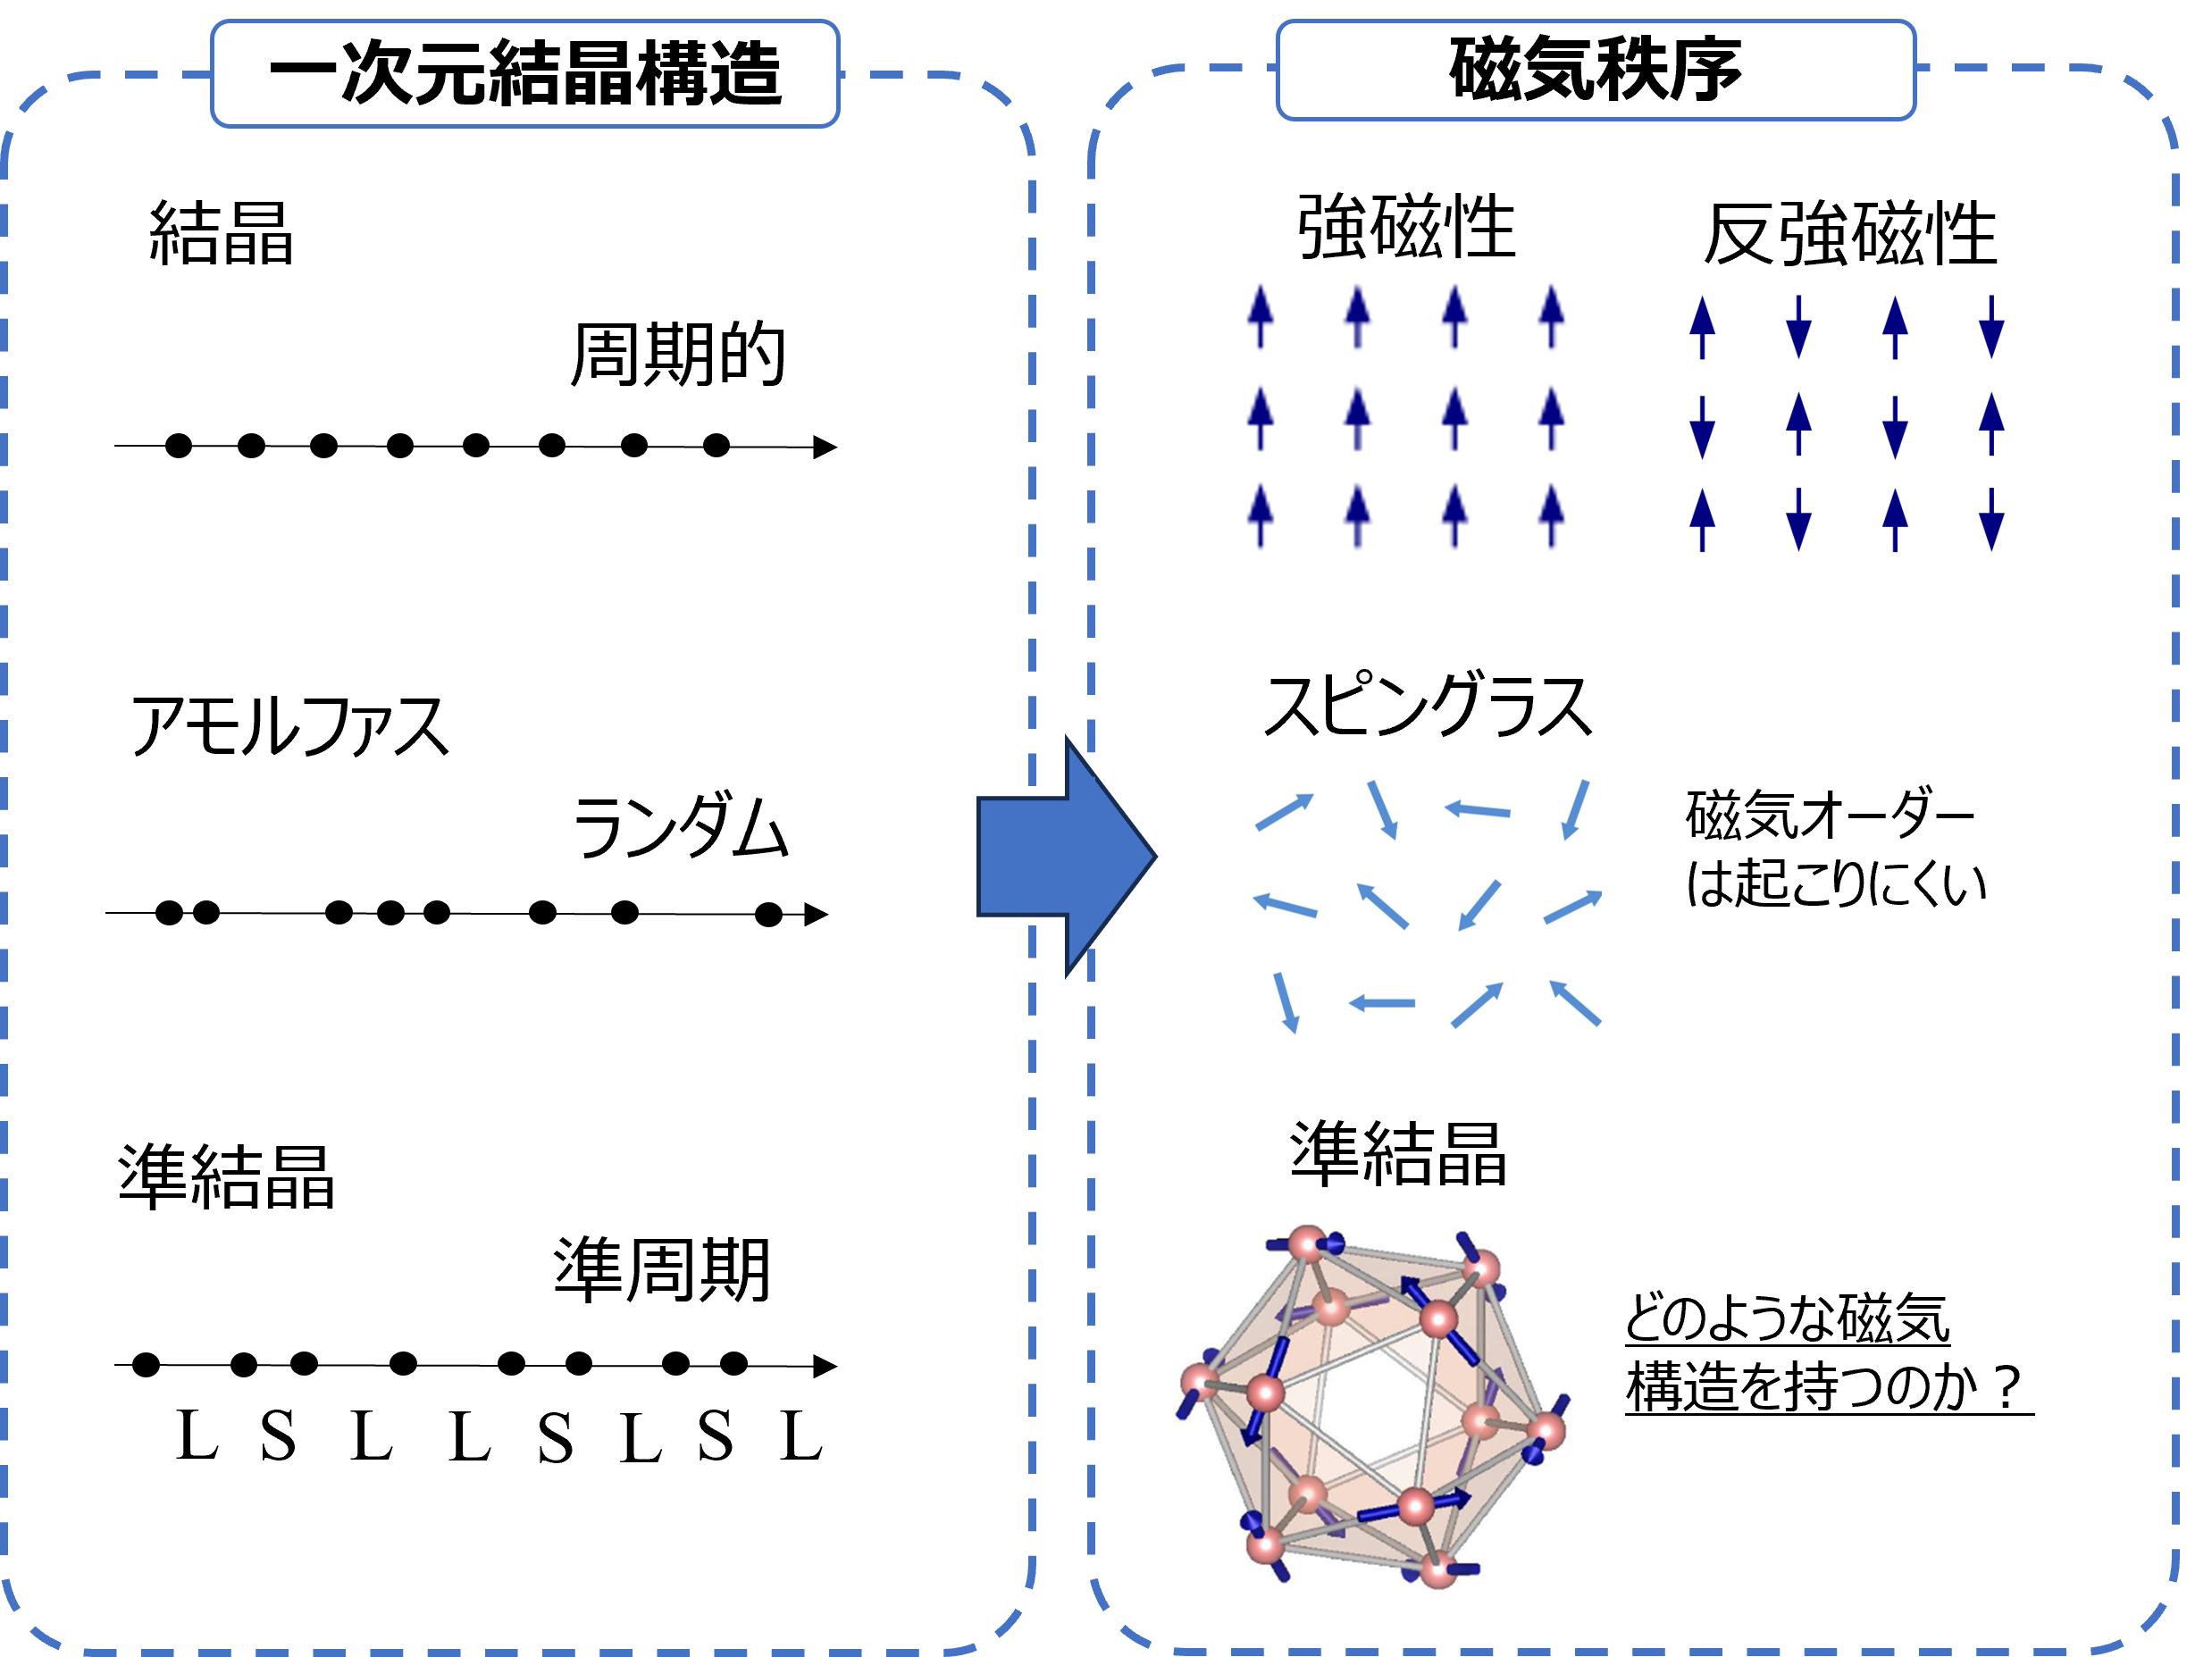
\includegraphics[width=140mm]{./figure/purpose_of_research.png}
  \caption{研究目標}
  \label{purpose_of_research}
\end{figure}
\chapter{準結晶}
\section{準結晶の定義}\label{準結晶の定義}
準結晶は、1章でも紹介した通り、通常の結晶が持つ原子配列秩序とは異なる新しいタイプの原子配列秩序を持った個体物質である。一般に固体の原子配列秩序、とくに長距離秩序、すなわち最近接原子間距離に比べて十分長い距離にわたって存在する秩序は、
X線や電子線の回折スペクトルに端的に現れる。ここで、個体に入射した平面波が固体中の原子により散乱される場合を考える。電子密度を与える関数を$\rho({\bm r})$とし、散乱ベクトルを$\bm S$すると散乱波の足し合わせ$F(\bm S)$は
\begin{equation}
  F(\bm S)=\int{\rho(\bm r)} \exp (-2\pi i \bm S\cdot\bm r)d\bm r
\end{equation}
で表される。ここで、$\bm r$が張る空間が実空間なのに対して、$\bm S$が張る空間を逆空間という。\\
さらに散乱強度$I(\bm S)$は、
\begin{equation}
  I(\bm S) =  |F(\bm S)|^2
\end{equation}
で与えられる。$I(\bm S)$の性質は秩序性の観点から個体を分類する。\par
もし、個体がアモルファス(非結晶)なら、散乱強度$I(\bm S)$は連続的な関数となり、これは長距離秩序を持たないことを意味する。一方、個体が「広義の結晶」である場合$I(\bm S)$は、$\delta$関数のセットとなり
\begin{equation}
  I(\bm S) =  \sum_{i}{|A_i|^2\delta(\bm S- \bm G_i)}
\end{equation}
の回折スペクトルとなる。ここで、$\delta$の位置の集合${\bm G_i}$は逆格子である。
逆格子{$\bm G_i$}のあらゆる要素がある有限個のベクトルの組$\bm a_i^*(i=1,2,\cdots,N)$の整数線形結合で表せるとき、$a_i^*$を逆格子基本ベクトルという。最小の逆格子基本ベクトルの数を$N$とすると、並進対称性をもつ「狭義の結晶」では、その数$N$は空間の次元数$d$と一致する。一方、$N>d$となる「非周期結晶」の場合、空間次元の周期性を持たない、もし$N$が空間次元数より大きければそれは「非周期結晶」とよばれる。\par
また、2次元または3次元の「狭義の結晶」に許される回転対称性は2,3,4,6回に限られる。すなわち、それら以外の回転対称性は2次元、3次元の周期性と両立しない。しかし、「非周期結晶」ではその限りではなく、なかでも$I(\bm S)$が「狭義の結晶」に存在しない回転対称性、すなわち2,3,4,6回以外の回転対称性をもつ場合、そのような構造を「準結晶」とよび、そうでないものを「非整合結晶」と呼ぶ。
\section{準結晶格子}
\ref{準結晶の定義}節の準結晶の定義を満たす構造のなかで、少数個の単位胞の充填構造からなるものを一般に「準結晶格子」とよぶ。準結晶格子は、実際の準結晶物質の原子配列構造記述する上で重要な役割を果たすものである。本節では、典型的な準結晶格子である2次元ペンローズ格子、3次元ペンローズ格子について説明する。しかし、その前に、厳密には「準結晶格子」とはいえないが、2次元、3次元のペンローズ格子と密接に関系する1次元フィボナッチ格子について説明する。1次元フィボナッチ格子は次元が低いので、準結晶格子やそのフーリエ変換の一般的な記述法、またそれらに関連する重要な概念を記述するのに適している。
\begin{figure}[htbp]
  \centering
  \vspace{10mm}
  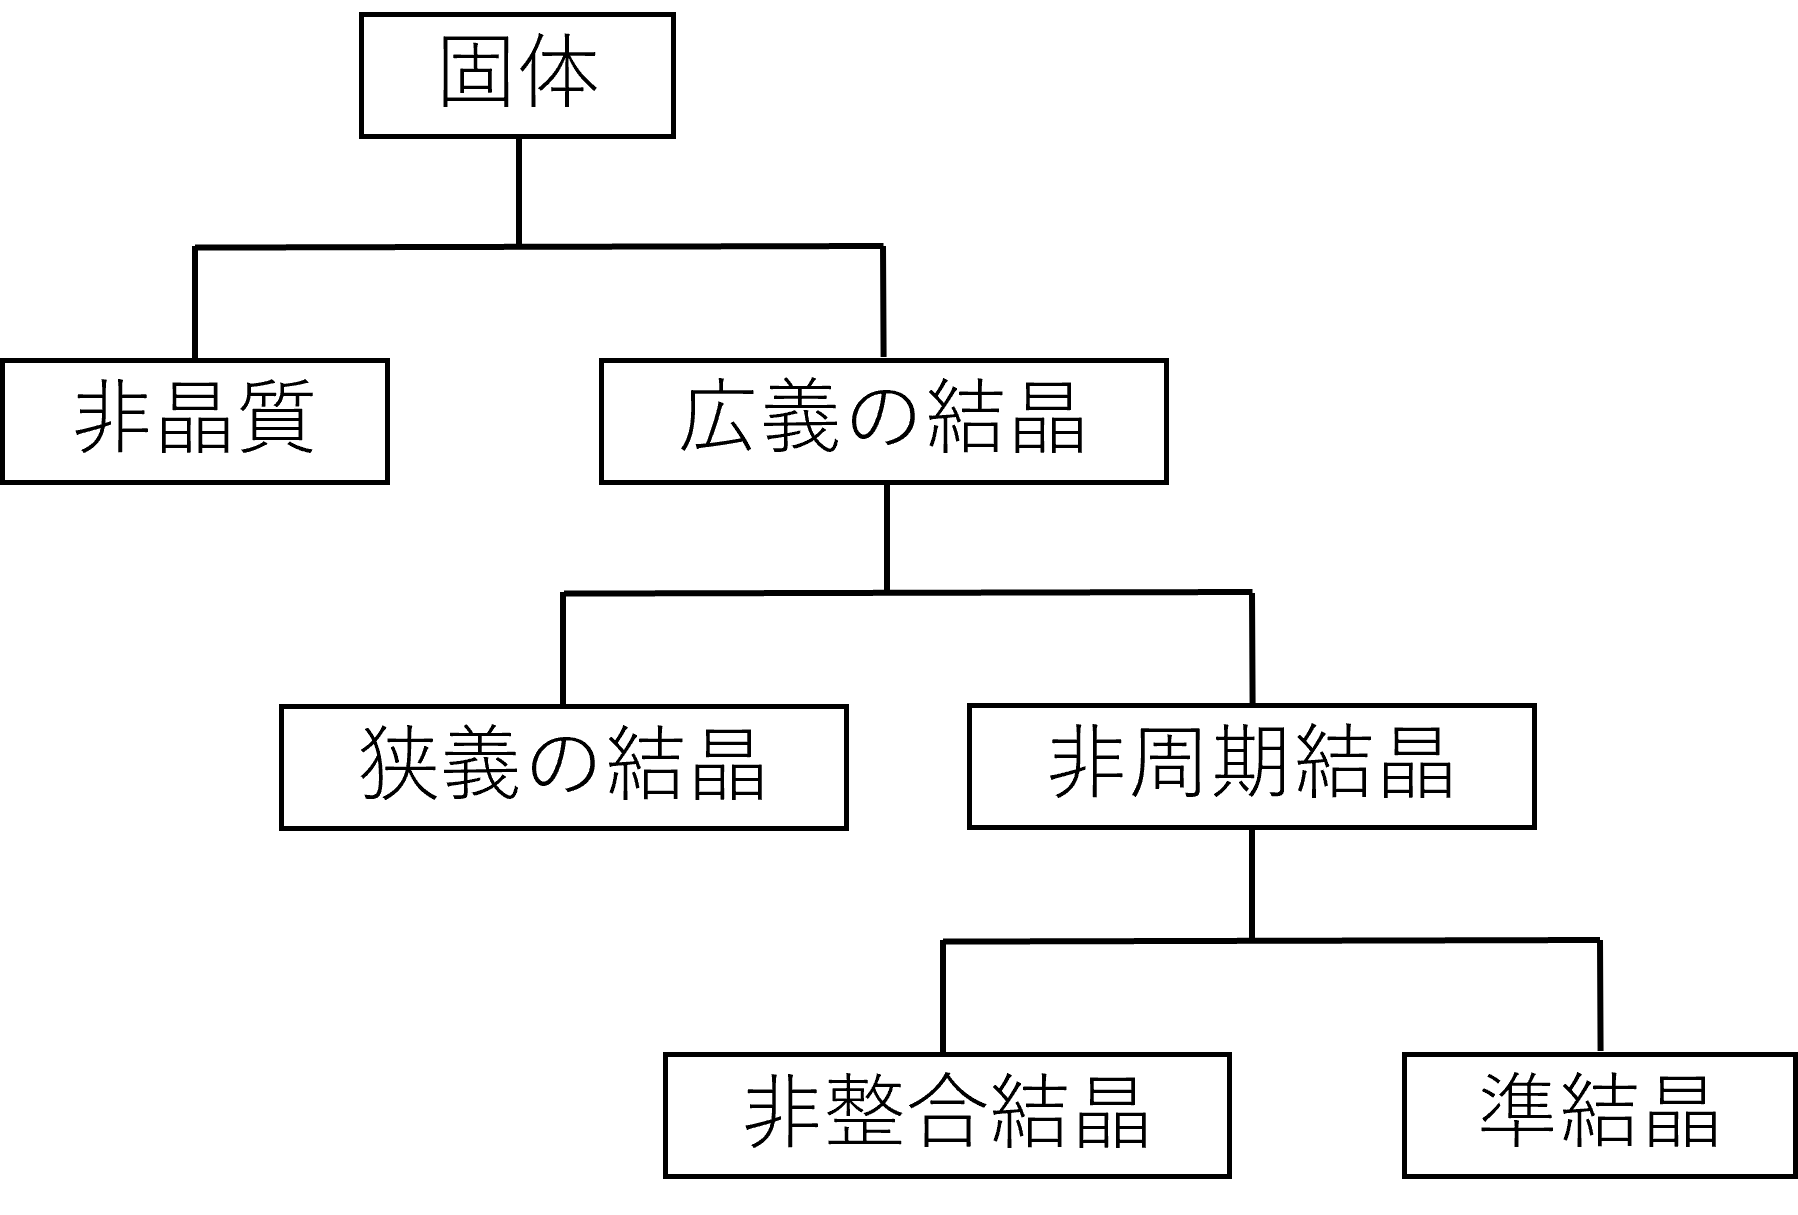
\includegraphics[width=120mm]{./figure/quasicrystalline_define.png}
  \caption{準結晶の定義}
  \label{quasicrystalline_define}
\end{figure}
\subsection{1次元フィボナッチ格子}
1次元においては\ref{準結晶の定義}でも説明した準結晶の定義である1,2,3,4,6以外の回転対称性を持っているという構造が存在しないので、厳密には1次元準結晶格子というものは存在しない。しかし、少数個の単位胞からなる1次元準周期構造は存在するので、ここではこれらを「1次元準周期格子」と呼ぶことにする。1次元準周期格子のような構造は、2次元の典型的な準結晶格子である2次元の典型的な準結晶格子である2次元ペンローズ格子や、後述する3次元の典型的な準結晶格子である3次元ペンローズ格子の中に見出すことができるので、それらの構造を理解する上で重要である。特に黄金比$\tau=(1+\sqrt5)/2$の基本長さの比をもつ1次元準周期格子「フィボナッチ格子」の構造は2次元、3次元のペンローズ格子の構造と密接に関係している。ここではこのフィボナッチ格子について述べる。\par
フィボナッチ格子は長さの比が$\tau$の2種類の間隔LとS(longとshotの意味)がいわゆるフィボナッチ配列をした構造を持つ。フィボナッチ配列は次のように定義される。まず、Lを第1世代としてこれを$\tau:1$に内分すると第2世代の配列LSが得られる。これのLをさらに$\tau:1$に内分すると第3世代のLSLが得られる。ここで第2世代のSの長さを1とすると第2世代のLは$\tau$であり、これを$\tau:1$に内分すると$\tau\cdot\tau/(\tau+1)$の2つの長さが生ずる。$\tau^2=\tau+1$なのでこれらは1と$1/\tau$になり、第2世代のSはそのまま第3世代のLになる。このような変換を無限に繰り返すことにより、図\ref{fibonacci_lattice}に示すような、LとSからなるフィボナッチ格子が得られる。この作り方から、フィボナッチ格子が$\tau$倍のスケール変換に関する自己相似性をもつことがわかる。
\begin{figure}[htbp]
  \centering
  \vspace{10mm}
  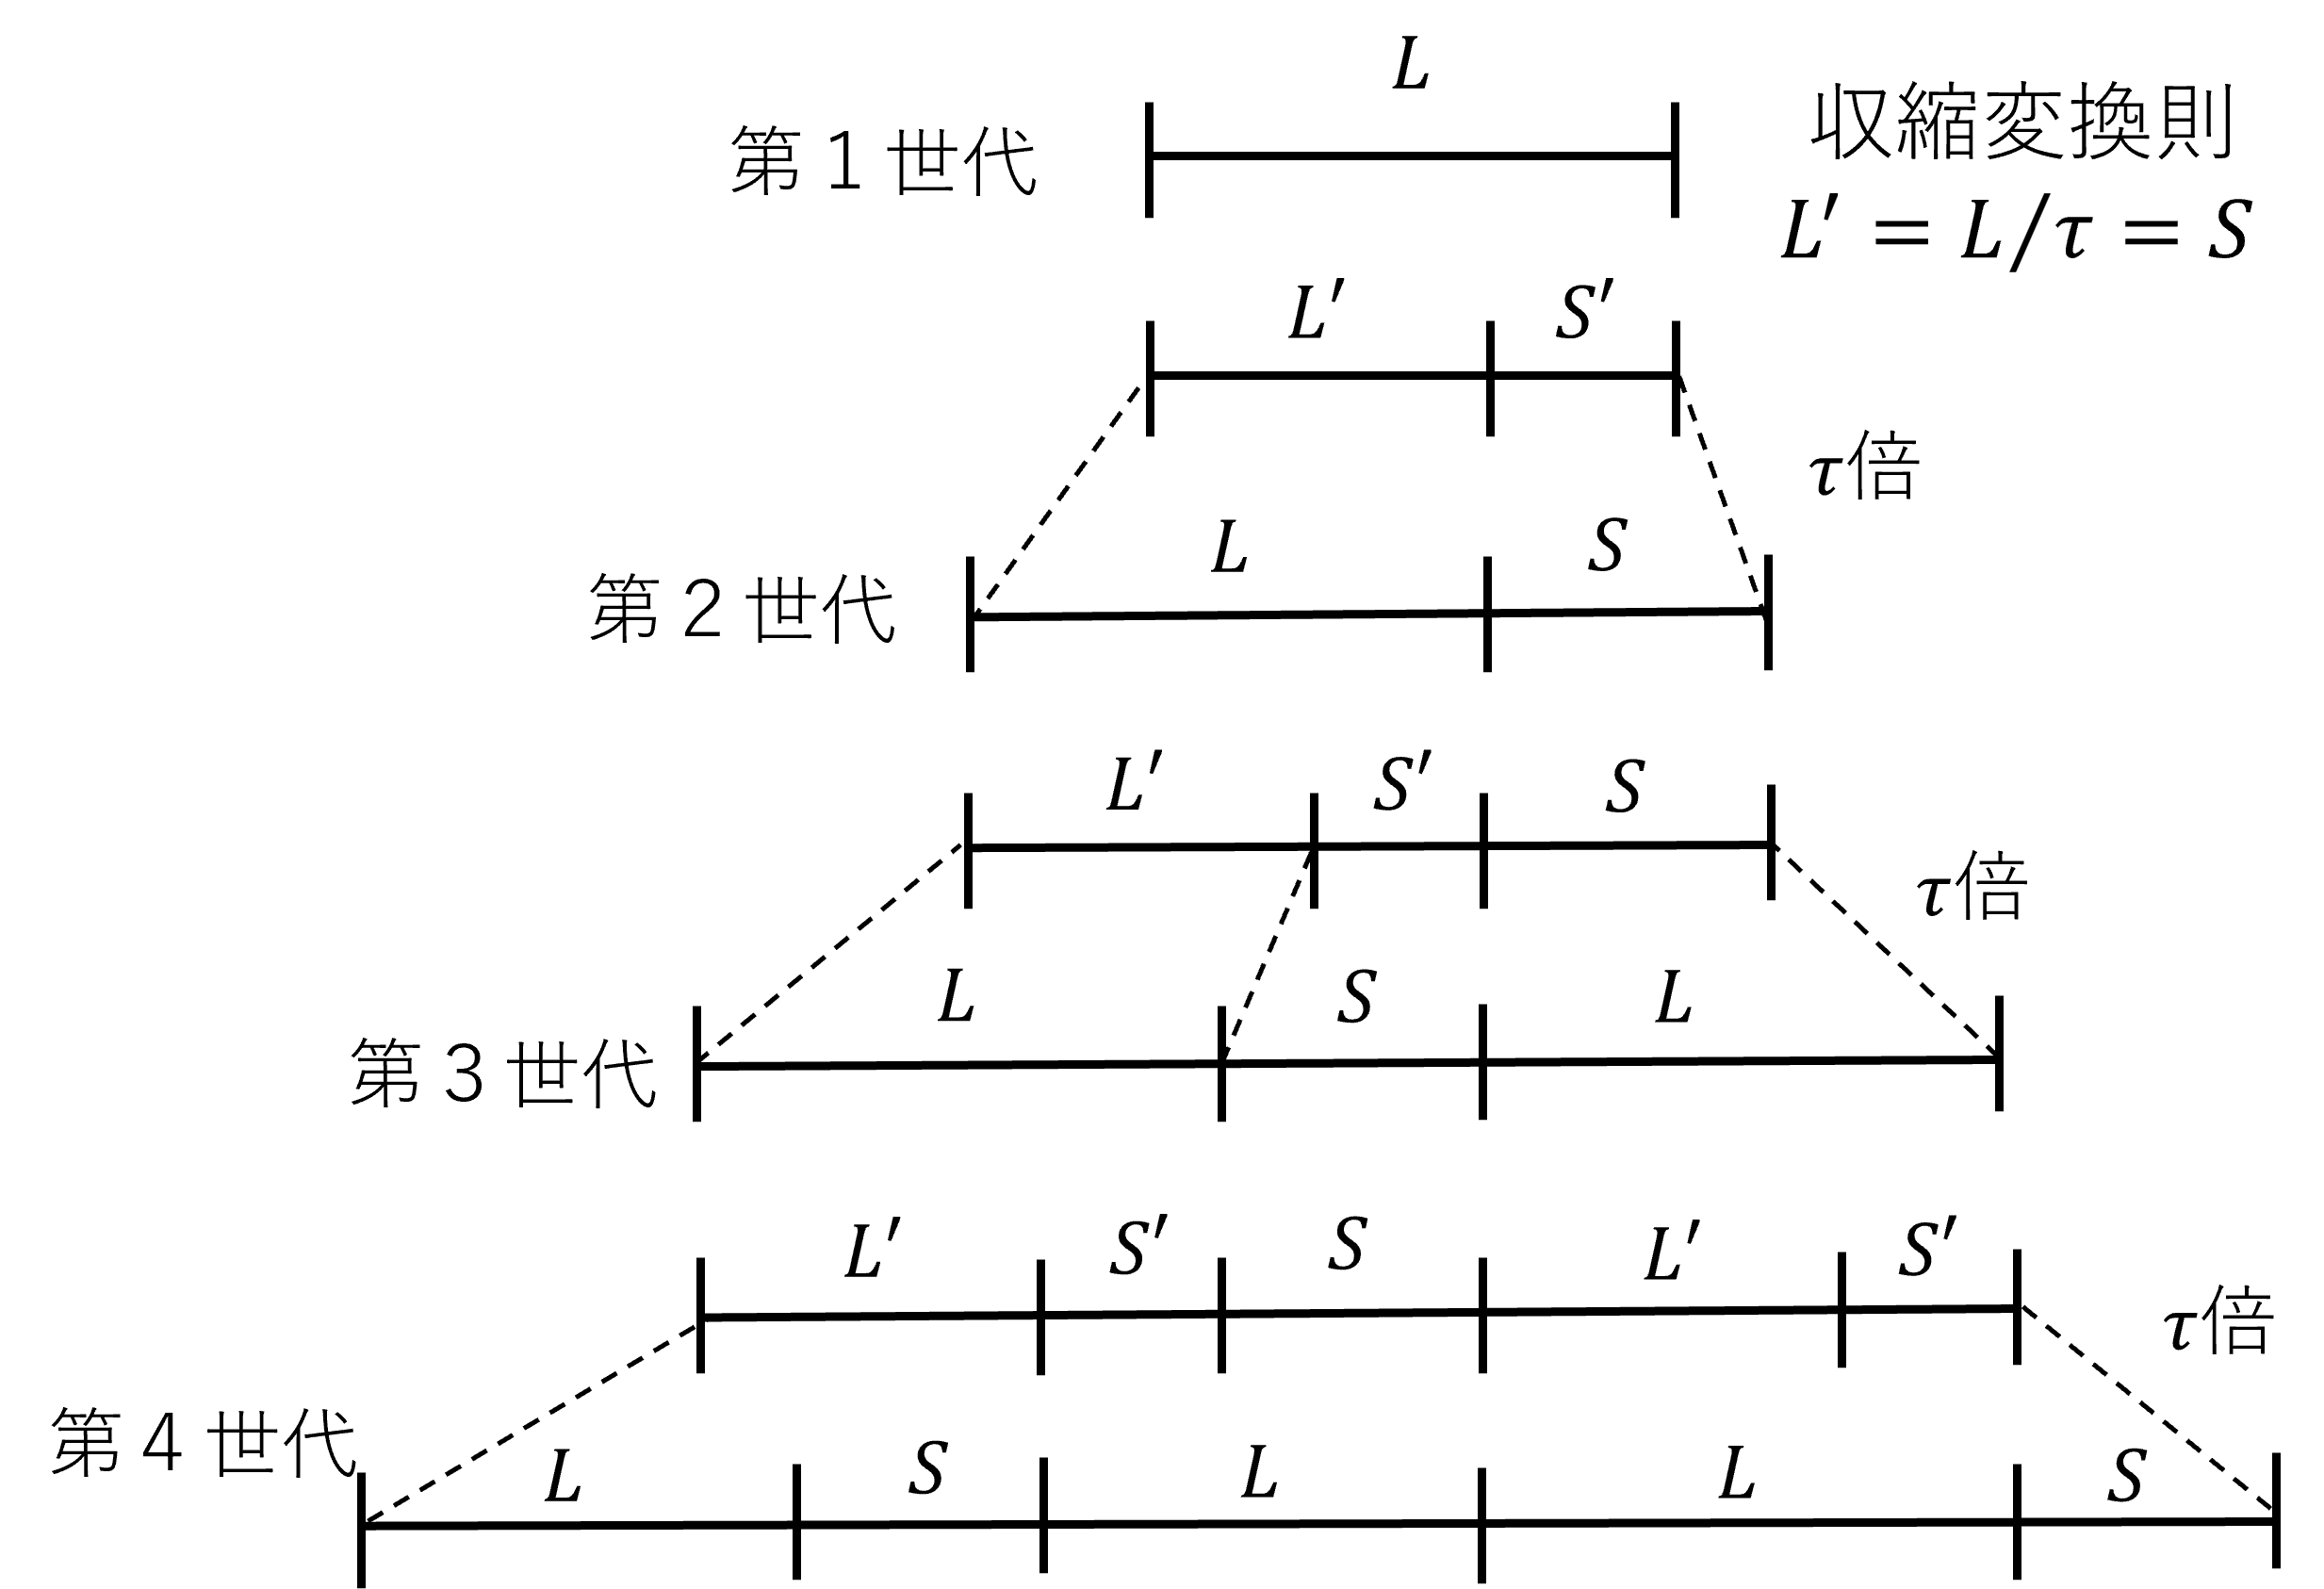
\includegraphics[width=120mm]{./figure/fibonacci_lattice.png}
  \caption{フィボナッチ格子}
  \label{fibonacci_lattice}
\end{figure}
フィボナッチ配列では第$n$世代$(n\ge3)$は、第$(n-1)$世代の後ろに第$(n-2)$世代をくっつけたものになっている。第$n$世代のLとSの総数を$F_n$とおくと、このような関係から
\begin{equation}
  F_n = F_{n-1}+F_{n-2}\quad (n\ge3)
\end{equation}
が成り立つ。$F_1=1,F_2=2$としてこの漸化式で定義される数列$1,2,3,5,8,13,\cdots$はフィボナッチ数列よばれる。




\subsection{2次元ペンローズ格子}
2次元準結晶格子には5,8,10,12回の回転対称性をもつものが存在する。なかでも、回折パターンに10回回転対称性を持つ準結晶格子は2次元ペンローズ格子と呼ばれる代表的な準結晶格子である。この格子は、2種類の菱形(厚い菱形と薄い菱形)を特定のタイル張りルールに従って構成され、各タイルは角度が72度と36度を持ち、黄金比$\tau=(1+\sqrt{5})/2$に関連にした寸法を有する。さらにペンローズ格子は自己相似性を特徴とし、拡大や縮小を行っても同様のパターンが現れる。これはスケール不変性と呼ばれ、準結晶の特性の一つである。
また、2次元ペンローズ格子とその回折像は、フーリエ変換で結ばれており、5回回転対称性をもつ2次元ペンローズ格子をフーリエ変換すると10回回転対称性をもつ回折像になり、逆に回折像からフーリエ逆変換をすることにより、実空間における2次元ペンローズ格子が得られる。
\begin{figure}[htbp]
  \centering
  \vspace{3mm}
  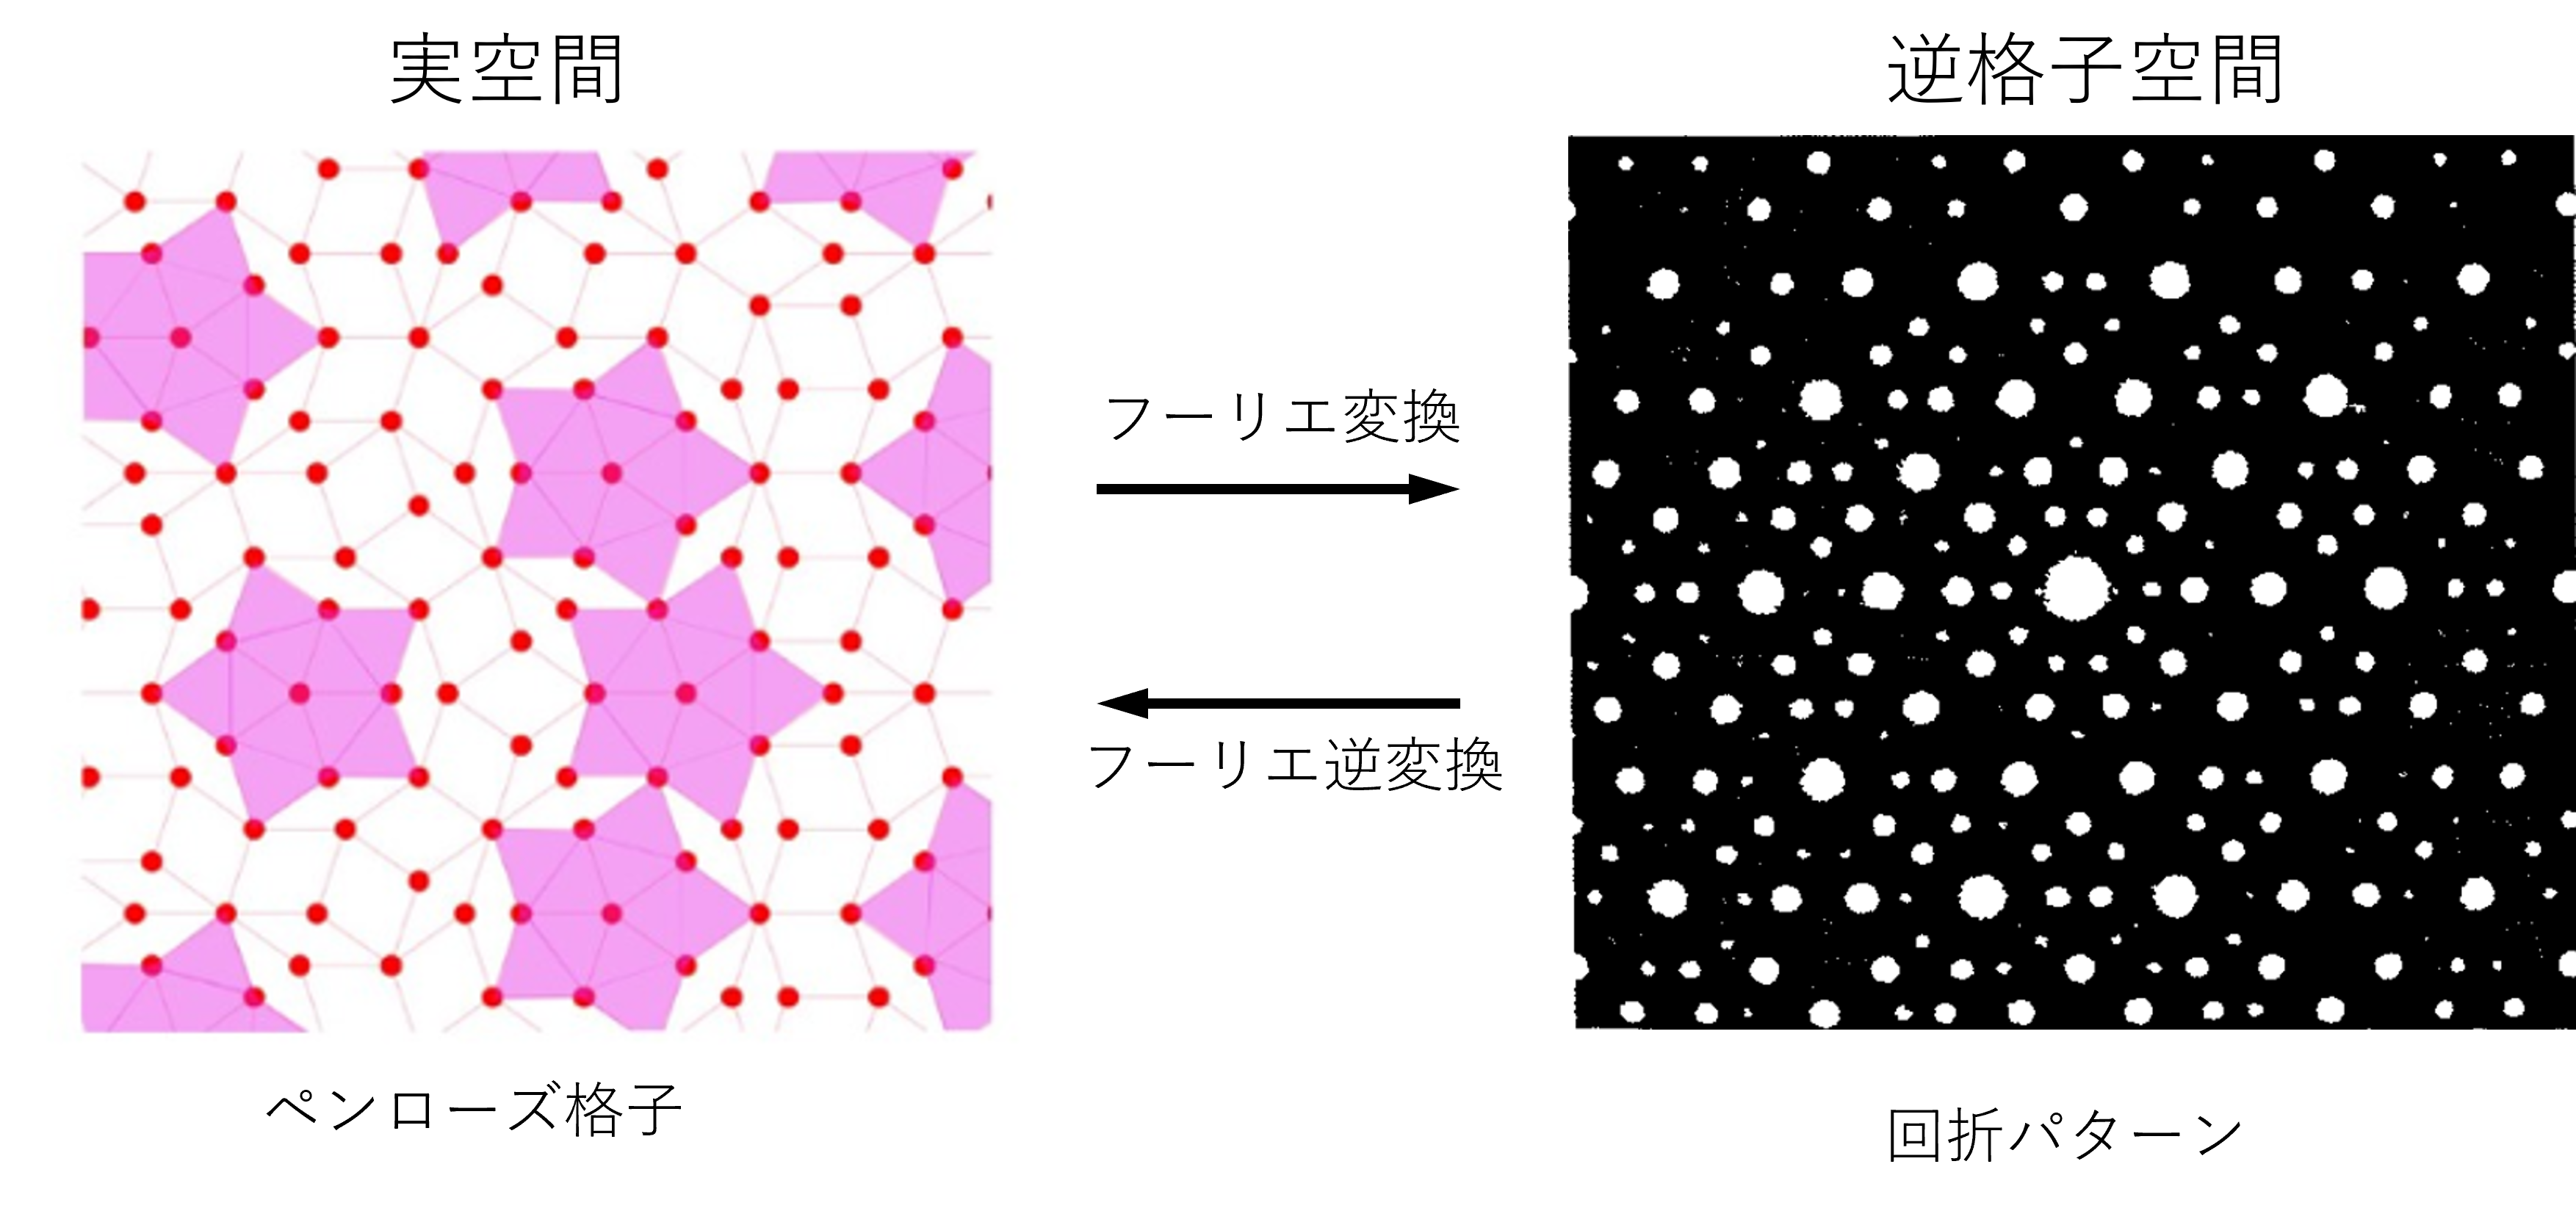
\includegraphics[width=150mm]{./figure/penrose_tile.png}
  \caption{2次元ペンローズ格子と回折像}
  \label{penrose_tile}
\end{figure}

\subsection{3次元ペンローズ格子}
3次元ペンローズ格子は、5次元空間で正20面体対称性を持つ周期的な格子を3次元空間に射影することで得られる特殊な構造である。高次元の周期的な格子から適切な部分を選び出し、それを低次元の物理空間に射影することで、非周期的でありながら秩序だったパターンを形成することができる。この5次元から3次元への射影過程では、正20面体の対称性は維持され、ペンローズ格子にもこの特異な対称性が反映される。結果として、通常の周期的な格子では実現できない5回対称性などの特徴が現れ、ペンローズ格子の非周期性と長距離秩序を説明することができる。

\subsection{高次元投影法}\label{高次元投影法}
高次元の周期的な格子構造を利用して、低次元での準周期的な構造を生成する方法を高次元投影法と呼ぶ。これにより、高次元空間でのシンプルな構造を低次元に投影することで複雑な準周期構造を理解することに役立つ。ここでは、1次元準周期格子を例にあげ、高次元投影法について説明する。
1次元準周期構造の回折関数$F(\bm S)$は、長さの比が黄金比$\tau$になる2つの基本逆格子ベクトル$\bm a_1^*,\bm a_2^*$を用いて表すことができ
\begin{equation}
  F(\bm S) = \sum_{n_1}\sum_{n_2}{A_{n_1,n_2}\delta(S-(n_1\bm a_1^*+n_2\bm a_2^*))}
  \label{F_S}
\end{equation}
となる。これをフーリエ逆変換して逆空間の関数$F(\bm S)$から実空間の関数$\rho(\bm r)$に直すと
\begin{equation}
  \rho(\bm r)=\sum_{n_1}\sum_{n_2}{A_{n_1,n_2}\exp[2\pi i(n_1\bm a_1^*+n_2\bm a_2^*)\cdot\bm r]}
  \label{rho_r}
\end{equation}
となる。このような1次元準周期構造は、ある2次元周期関数の1次元断面として記述できることが以下のようにしてわかる。まず式(\ref{rho_r})に対して関数$\rho^h(t_1,t_2)$($h$は高次元関数または高次元ベクトルを表す添え字)を次式で定義する。
\begin{equation}
  \rho^h(t_1,t_2)=\sum_{n_1}\sum_{n_2}{A_{n_1,n_2}\exp[2\pi i(n_1t_1+n_2t_2)]}
  \label{rho_t}
\end{equation}
これは、$t_1,t_2$に関して周期1の周期関数になっている。式(\ref{rho_r}),式(\ref{rho_t})より
\begin{equation}
  \rho(\bm r)=\rho^h(t_1,t_2)
  \label{rho_r_t}
\end{equation}
ただし,
\begin{equation}
  \left\{
    \begin{aligned}
      t_1 = \bm a_1^*\cdot\bm r \\
      t_2 = \bm a_2^*\cdot\bm r
    \end{aligned}
 \right.
\end{equation}
ここで$\bm a_1^*,\bm a_2^*$の比から
\begin{equation}
  t_2=\tau t_1
  \label{t_t}
\end{equation}
である。このことから、1次元準周期関数$\rho(\bm r)$が2次元周期関数$\rho^h(t_1,t_2)$の式\ref{t_t}であらわされる直線上の値として得られることがわかる。\par
図\ref{High_dimensional_projection}にこのような形で記述した1次元準周期構造の例を示す。基本周期ベクトル$\bm d_1,\bm d_2$を図のように$|\bm d_1|=|\bm d_2|,\bm d_1\perp \bm d_2$をみたすようにとる。ここで、2次元空間内で関数$\rho(\bm r)$が得られる1次元部分空間を$E_\parallel$,それと直交する補空間を$E_\perp$と名付ける。2次元周期関数としては各格子点に$E_\perp$方向に伸びた線分がくっついたものを考えており、この関数は線分上でのみ$\delta$関数的に値をもち、他では値が0である。よって、$E_\parallel$上の1次元密度関数$\rho(\bm r)$は、2次元周期関数との交点で値を持つ$\delta$関数のセットからなり、さらに$\delta$関数の長さには適当な下限と上限があるので、実際の原子配列の1次元的なモデルになりうるものである。$E_\perp$方向にのびた線分が$E_\parallel$と交差する点が$E_\parallel$上で原子位置に対応し、この線分は高次元空間(hyperspace)の原子という意味で「超原子」(hyperatom)とよばれる。
\begin{figure}[htbp]
  \centering
  \vspace{3mm}
  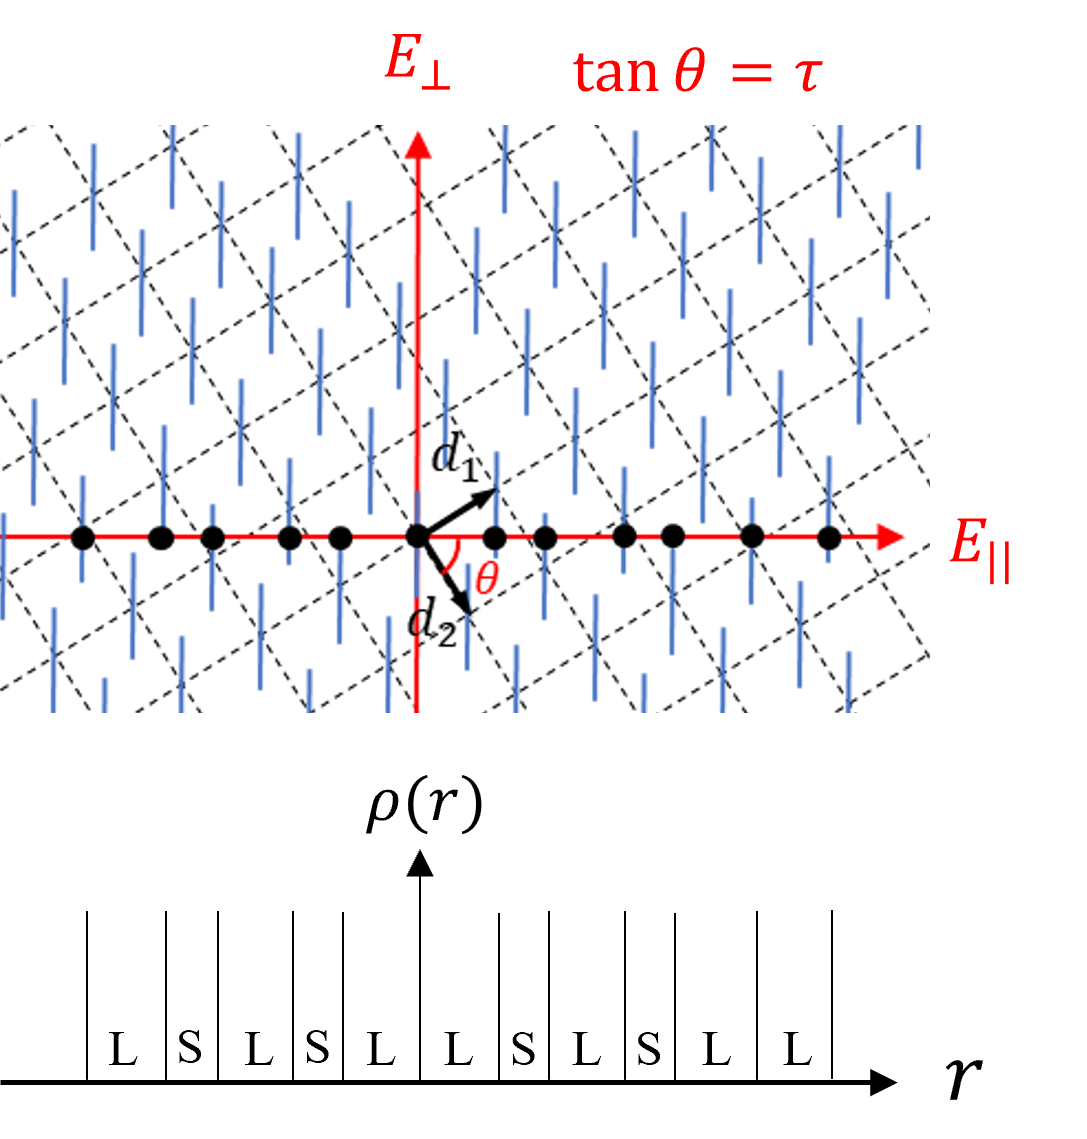
\includegraphics[width=100mm]{./figure/High_dimensional_projection.png}
  \caption{高次元投影法}
  \label{High_dimensional_projection}
\end{figure}
\section{近似結晶}
近似結晶は、準結晶と密接な関係を持ちながら、周期的な結晶構造を有する物質である。準結晶は、従来の結晶学の枠組みでは禁じられていた対称性、例えば五回回転対称性や十回回転対称性を示す非周期的な構造を持つことで知られているが、近似結晶はこれらの準結晶と類似した局所的な原子配置や対称性を持ちつつ、全体としては周期的な構造を維持している。この周期性は、大きな単位胞内に多数の原子が配置され、その単位胞が空間内で周期的に繰り返されることにより実現している。\par
近似結晶の形成には、フェイゾン歪と呼ばれる特殊な歪みが関与している。フェイゾン歪は、準結晶における追加の自由度であるフェイゾン自由度に起因し、この歪みを導入することで非周期的な準結晶構造が周期的な結晶構造に変換される。一次元の準結晶モデルであるフィボナッチ格子において、フェイゾン歪を導入すると、\ref{高次元投影法}節の高次投影法において逆格子ベクトルの比が有理数(つまり、$\tan \theta$が有理数)となり、投影された格子の関数$\rho(r)$は周期的になる。この有理数の比はフィボナッチ数列に関連し、例えば逆格子ベクトルの比が $1/1, 2/1, 3/2,\dots,F_{n+1}/F_n$ となると、1周期内の配列もLS,LSL,LSLLS,…のように増えていき、$n$の値が多きくなるにつれて準結晶構造に近くなる。ここで、$1/1$ の場合は 1/1 近似結晶、$2/1$ の場合は 2/1 近似結晶と呼ばれる。\par
また、近似結晶の研究は、準結晶の複雑な構造や物理的性質の解明において重要な役割を果たす。準結晶はその非周期的な構造のために直接的な解析が難しいが、周期構造を持つ近似結晶を解析することで、準結晶の構造に関する間接的な情報が得られる。特に、近似結晶の原子配列や対称性、電子構造などを調べることで、準結晶における物理的特性の予測や理解が進むと考える。

\begin{figure}[htbp]
  \centering
  \vspace{10mm}
  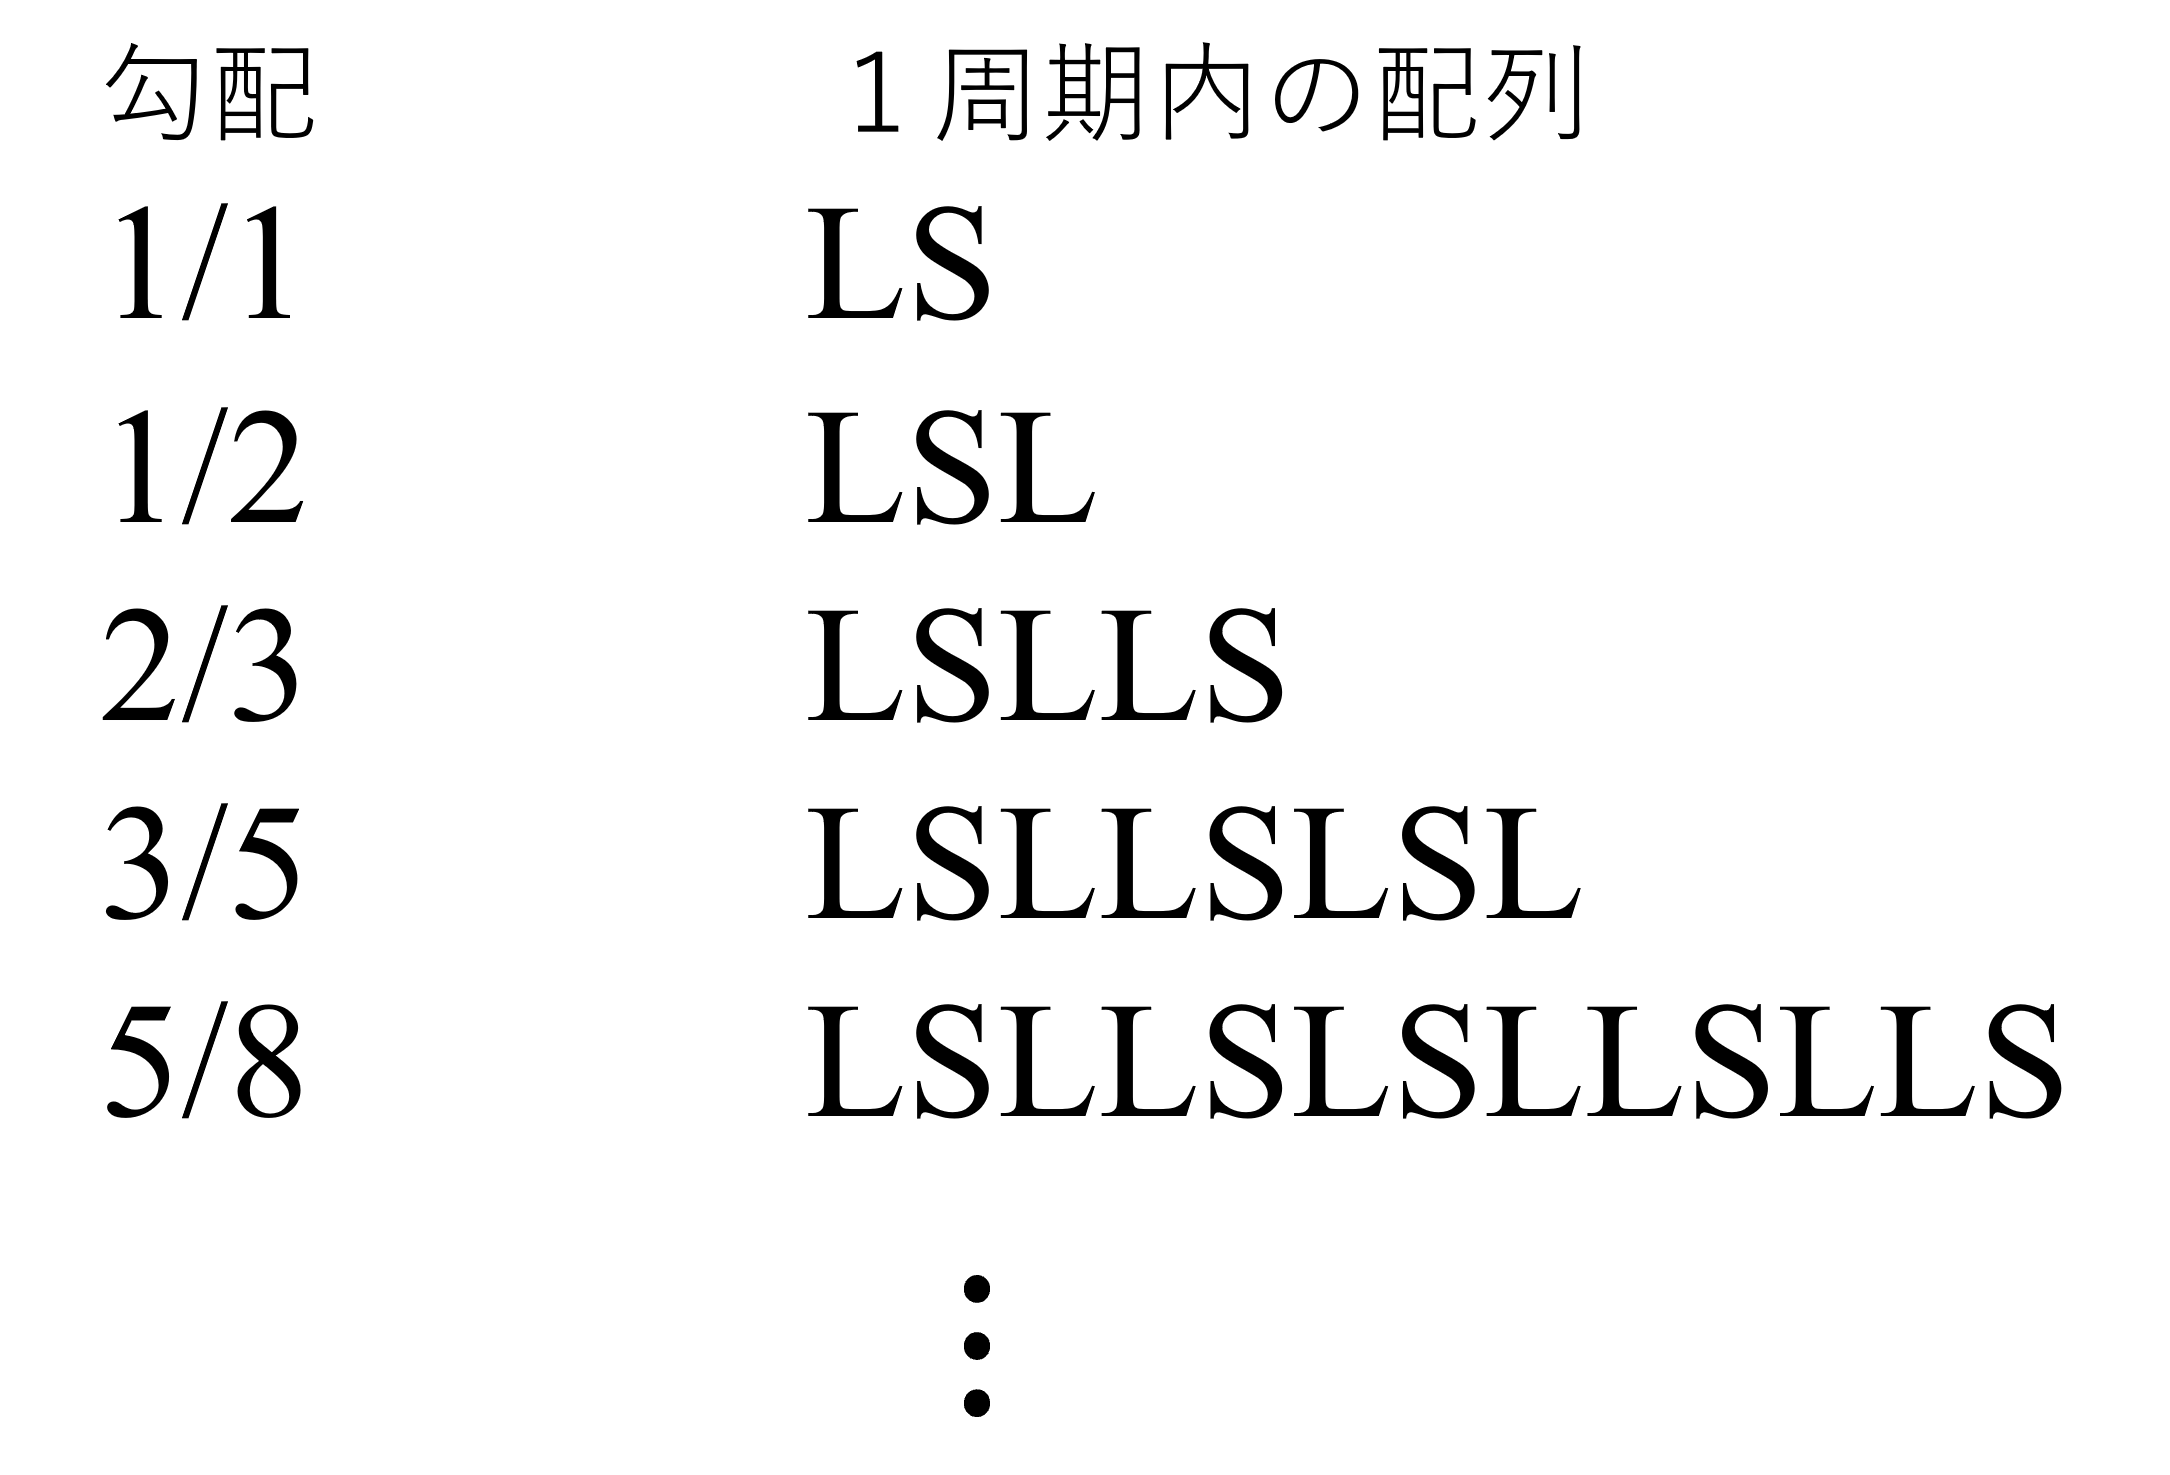
\includegraphics[width=100mm]{./figure/LS.png}
  \caption{逆格子ベクトルの比と1周期内の配列}
  \label{LS}
\end{figure}

\chapter{NMRの原理}
\section{核磁気共鳴現象}

\section{超微細相互作用}
超微細相互作用は、核磁気モーメント$\bm \mu_n$と電子の相互作用であり、NMRやNQRなどの共鳴型磁気測定において極めて重要な役割を果たす。この相互作用は、共鳴線のシフトや核スピンの緩和過程に影響を与えるため、物質のミクロな電子状態を理解するための手がかりとなる。\par
原点に核磁気モーメント$\bm \mu_n$を置き、電子の座標を$\bm r$とする。$\bm \mu_n$による点$\bm r$におけるベクトルポテンシャル$\bm A(\bm r)$は
\begin{equation}
  \bm A(\bm r)=\nabla\times \frac{\bm \mu_n}{r}
\end{equation}
である。電子の運動量$\bm p$およびスピン$\bm s$との相互作用のハミルトン二アンは
\begin{equation}
  \mathcal{H} = \frac{1}{2m}\left(\bm p + \frac{e}{c}\bm A(\bm r)\right)^2 + 2\mu_{\text B} \bm s\cdot\nabla\times\bm A
  \label{H}
\end{equation}
であり、$\bm A(\bm r)=0$からの差は
\begin{align} 
    \mathcal{H}_l&=\frac{e}{2mc}(\bm p\cdot \bm A+\bm A\cdot\bm p+\frac{e}{c}\bm A^2)+2\mu_{\text B}\bm s\cdot\left(\nabla\times\left(\nabla\times\frac{\mu_n}{r}\right)\right)\\
    &=\mathcal{H}_l+\mathcal{H}_s+\frac{e^2}{2mc^2}\bm A^2
\end{align}
となる。ここで、
\begin{equation}
  \mathcal{H}_l=\frac{e}{2mc}(\bm p\cdot\bm A + \bm A \cdot \bm p)
  \label{H_l}
\end{equation}
\begin{equation}
  \mathcal{H}_s=2\mu_{\text B}\bm s\cdot\left(\nabla\times\left(\nabla\times\frac{\mu_n}{r}\right)\right)
  \label{H_s}
\end{equation}
まず、式(\ref{H_l})の$\mathcal{H}_l$について考える。
\begin{equation}
  \bm A(\bm r)=\nabla\times\frac{\bm \mu_n}{r}=\frac{\bm \mu_n\times\bm r}{r^3}
\end{equation}
であるから、
\begin{equation}
  \mathcal{H}_l=\frac{e}{2mc}\left(\bm p\cdot\frac{\bm{\mu}_n\times\bm{r}}{r^3}+\frac{\bm{\mu}_n\times\bm{r}}{r^3}\cdot\bm{p}\right)
\end{equation}
となり、$\bm{r}\times\bm{p}=\hbar\bm{l}$、$\mu_{\text B}=e\hbar/2mc$をつかって
  \begin{align}
    \mathcal{H}_l&=2\mu_{\text B}\frac{\bm{I}\cdot\bm{l}}{r^3}\\
    &=\gamma_e\gamma_n\hbar^2\frac{\bm{I}\cdot\bm{l}}{r^3}
    \label{H_orb}
  \end{align}
となる。これは核スピンと電子の軌道角運動量との相互作用で、$l\leq1$の$p,d,f,\cdots$電子が関与する。\par
次に、式(\ref{H_s})の$\mathcal{H_s}$は、核スピンと電子スピンの相互作用であるが、
\begin{equation}
  \nabla \times \left( \nabla \times \frac{\bm{\mu}_n}{r} \right) = \nabla\left( \nabla \cdot \frac{\bm{\mu}_n}{r} \right) - \Delta \frac{\bm{\mu}_n}{r}
\end{equation}
を用いると、
\begin{equation}
  \mathcal{H}_s=2\mu_{\text B}\left[(\bm{s}\cdot\nabla)(\mu_n\cdot\nabla)\frac{1}{r}-\frac{1}{3}\bm{s}\cdot\Delta\frac{\mu_n}{r}\right]-\frac{4}{3}\mu_{\text B}\bm{s}\cdot\Delta\frac{\bm{\mu}_n}{r}
  \label{H_s_2}
\end{equation}
となる。第1項は
\begin{align}
  \mathcal{H}_s^1 &= 2 \mu_{\text B} \sum_{i,j} s_{x_i} \frac{\partial^2}{\partial x_i \partial x_j} \mu_{n x_j} \left( \frac{1}{r} \right) - \frac{1}{3} s_{x_i} \mu_{n x_i} \frac{\partial^2}{\partial x_j^2} \left( \frac{1}{r} \right)\\
  &=2\mu_{\text B} \sum_{i,j} s_{x_i} \mu_{n x_j} \Lambda_{ij}
\end{align}
\begin{align}
  \Lambda_{ij} &= \frac{1}{3} \left(3 \frac{\partial^2}{\partial x_i \partial x_j} - \delta_{ij} \sum_k \frac{\partial^2}{\partial x_k^2} \right) \left( \frac{1}{r} \right)\\
  &= \frac{1}{3} \frac{3x_i x_j - r^2 \delta_{ij}}{r^5}
\end{align}
と書かれる。ここで$x_1,x_2,x_3$は$x,y,z$を表す。$r\neq0$では$\mathcal{H}_s^l$は磁気双極子相互作用
\begin{equation}
  -\frac{2\mu_{\text B}\bm{s}\cdot\bm{\mu}_n}{r^3}+\frac{3(\mu_{\text B}\bm{s}\cdot\bm{r})(\bm{\mu}_n\cdot\bm{r})}{r^5}
\end{equation}
であり、式\ref{H_s_2}第2項$\mathcal{H}_s^2$は0となる。一方、$r\to0$では
\begin{equation}
  \Delta \left(\frac{1}{r}\right)=-4\pi\delta(\bm{r})
\end{equation}
であるから
\begin{align}
  \mathcal{H}_s^2&=\frac{16}{3}\pi \mu_{\text B} \bm{s}\cdot\bm{\mu}_n|\psi_s(0)|^2\\
  &=\frac{8}{3}\pi \gamma_e\gamma_n\hbar^2|\psi_s(0)|^2\bm{s}\cdot\bm{I}
\end{align}
となり、$\mathcal{H}_s^1$が消える。以上の議論から、核スピンと電子スピンの相互作用$\mathcal{H}_s$は磁気双極子相互作用
\begin{equation}
  \mathcal{H}_{\text{dip}} = -\frac{\gamma_e \gamma_n \hbar^2}{r^3} \left\{ \bm{s} \cdot \bm{I} - \frac{3 (\bm{s} \cdot \bm{r}) (\bm{I} \cdot \bm{r})}{r^2} \right\}
  \label{H_dip}
\end{equation}
とフェルミの接触相互作用
\begin{equation}
  \mathcal{H}_F=\frac{8}{3}\pi\gamma_e\gamma_n\hbar^2\bm{s}\cdot \bm{I}\delta(r)
  \label{H_F}
\end{equation}
がある。$\mathcal{H}_{dip}$には$p,d,f,\cdots$電子が、$\mathcal{H}_F$には$s$電子が関与する。\par
$H_l,H_s$は基本的な相互作用であるが、間接的な相互作用として内殻偏極の相互作用がある。これは、電子スピンが分極すると交換相互作用により、内側の閉殻の電子スピンの空間分布が変化し、それにより核位置における内殻$s$スピンの電子密度が変化する。外側のスピンと平行な内殻$s$電子スピンの軌道は広がり、反平行スピンの核位置の密度が増え、外側スピンと核スピンの間に大きな相互作用が生じる。これは、
\begin{equation}
\mathcal{H}_{core}=\frac{8\pi}{3}\gamma_e\gamma_n\hbar^2\bm{I}\cdot\bm{s}\sum_{i}{(|\psi_i(0)|_\uparrow^2-|\psi_i(0)|_\downarrow^2 )}
\label{H_core}
\end{equation}
と書かれる。$s$は外側のスピンで$|\psi_i(0)|_{\uparrow,\downarrow }^2$は$i$番目の内殻$s$電子の上向き、下向きスピンの核位置での密度である。\par
また、同じ原子内の内殻偏極の効果と同様に、隣接イオンにおいても電子スピンの空間分布が変化し、核イオンと電子スピンとの間に新たな相互作用が生じることがある。この空間分布の変化は、不対電子の波動関数と隣接イオンの電子軌道が部分的に重なり合うことで生じる。この隣接イオンの電子の空間分布により隣接イオンの核スピンは相互作用が生じる。この相互作用はtransfer相互作用とよばれ
\begin{equation}
\mathcal{H}_{trans} = A\bm{I}\cdot\bm{s}
\end{equation}
で表せる。ここで、$A$はtransfer超微細結合定数、$\bm I$は隣接核の核スピン演算子、$\bm s$不対電子のスピン演算子である。さらに、不対電子スピンと隣接核サイトの間には、磁気双極子相互作用も存在する。\par
以上をまとめると、式(\ref{H_orb})、式(\ref{H_dip})、式(\ref{H_F})、式(\ref{H_core})の期待値を$\mu_n$で割って($-$)をつけると、各相互作用を通じて核スピンに働く超微細磁場が得られる。
\begin{equation}
  \bm{H}_{orb} = -\gamma_e\hbar \langle \bm{l} \rangle \langle \psi^*|\frac{1}{r^3}|\psi \rangle 
\end{equation}
\begin{equation}
  \bm{H}_{dip} = \gamma_e\hbar \left\langle \psi^* \left|\frac{\left\langle\bm{s}\right\rangle}{r^3}-3\frac{(\left\langle \bm s\right\rangle \cdot \bm r)\bm{r} }{r^5} \right| \psi \right\rangle
\end{equation}
\begin{equation}
  \bm{H}_F = -\frac{8}{3}\pi \gamma_e \hbar \langle \bm{s}\rangle |\psi(0)|^2
  \label{H_F_2}
\end{equation}
\begin{equation}
  \bm{H}_{core} = -\frac{8}{3}\pi \gamma_e \hbar \langle \bm{s}\rangle \sum_{i}{(|\psi_i(0)|_\uparrow^2-|\psi_i(0)|_\downarrow^2 )}
\end{equation}
\par
電子スピンあるいは軌道角運動量の方向は、一般にはNMR周波数に比べて非常に早く変化しているので、核スピンの受ける磁場はそれぞれの時間平均となる。
\section{共鳴線のシフト}
一般に物質の中では、外部磁場$H_0$での周波数$\omega$は
\begin{align}
  \omega &= \omega_0 + \Delta K \\
  &= \gamma(H_0+\Delta H)
\end{align}
のように、$\omega_0=\gamma H_0$よりシフトする。このシフトは、電子の軌道磁化が作る磁場と電子スピンによる磁気モーメントが作る磁場により、前節で述べた超微細相互作用を通して、余分の磁場$\Delta H$を作るからである。まず、非磁性、非金属物質でメインとなる化学シフトについて述べる。化学シフトとは分子内の核周囲の電子の遮蔽に起因し、主に共有結合や化学結合の性質によるものである。この場合$\left\langle s_z \right\rangle = 0$である。式(\ref{H})に外場$H_0$が加わると
\begin{align}
  \mathcal{H} = \frac{1}{2m}(\bm p + \frac{e}{c} \bm A_0 +\frac{e}{c} \bm A_n)^2\\
  \bm A_0 =\frac{1}{2}(\bm H_0 \times \bm r), \bm A_n = \frac{\bm{\mu}_n \times \bm r}{r^3}
  \label{che}
\end{align}
となる。このとき、式(\ref{che})の第2項と第3項の積からは反磁性シフトが、そして第1項と第2項、および第1項と第3項の積の2次摂動エネルギーから常磁性シフトが得られる。\par
ここで、反磁性シフトとは、磁場をかけると,ローレンツ力によって,その変化を打ち消すように,原子核の周りを運動する電子の軌道角運動量が変化することによって生じる小さい負のシフトである。これは反磁性効果と呼ばれ、非磁性の有機化合物や非金属化合物で観測される。\par
一方、常磁性シフトとは、自由な回転運動が束縛されて$\langle l \rangle =0$となっている電子の軌道角運動量が、外部磁場$H_0$にによって一部回復し、余分な磁場$\Delta H$を生じることで発生する正のシフトである。
\subsection{ナイトシフトと局所磁化率}
金属や磁性体の常磁性状態では,伝導電子や局在電子の磁化が外部磁場により誘起されるので,核位置に大きな磁場をつくる.ナイト(Knight)は金属銅中の銅(Cu)核の共鳴位置が$Cu_2O$に比べて0.23%という大きい
シフトを持つことを発見した.特に発見者に因んでナイトシフト(Knight shift) という。その後,種々の金属において同様の結果が得られた。磁気的な遷移金属,遷移金属化合物,希土類化合物では,大きな負のナイトシフトを示す。これは以下しめすように,$s$電子系,$d$電子系,および$f$電子系のナイトシフトは、電子スピン分極によるからである。
\subsubsection{$s$電子系}
ブロッホ関数を
\begin{equation}
  \phi_{\bm{k}}(\bm{r}) = u_{\bm{k}}(\bm{r}) e^{i \bm{k} \cdot \bm{r}}
\end{equation}
とすると、フェルミの接触相互作用の式(\ref{H_F})によるエネルギーは
\begin{equation}
  \Delta E = \sum_{\bm{k}, \sigma} \left\langle \phi_k^* \middle| \frac{8}{3 \pi} \gamma_e \gamma_n \hbar^2 \bm{s}_k \cdot \bm{I} \delta(\bm{r}) \middle| \phi_k \right\rangle
\end{equation}
である。ここで、\(\phi_{\bm{k}}(\bm{r})\) は単位体積で規格化されている。単位体積あたりのパウリの常磁性スピン磁化率を \(\chi_P\) とすると
\begin{equation}
  -\gamma_e\hbar \sum_{\bm{k},\sigma} \left\langle \phi_k^* \middle| s_{\bm{k}z} \middle| \phi_k \right\rangle = \chi_P H_0
\end{equation}
であるから
\begin{equation}
  \Delta E = -\frac{8}{3 \pi} \gamma_n \hbar I \chi_P H_0 | u_{k_F}(0) |^2
\end{equation}
となって、ナイトシフト \(K_s\) は
\begin{equation}
  K_s = \frac{\Delta H}{H_0} = - \frac{\Delta E}{\gamma_n \hbar I} \frac{1}{H_0} = \frac{8 \pi}{3} | u_{k_F}(0) |^2 \chi_P
  \label{K_s}
\end{equation}
電子間の相互作用を無視すると、\(\chi_P = 2 \mu_{\text B}^2 N(E_F)\) である。ここで \(N(E_F)\) はフェルミ面での単位体積あたりの1スピン状態密度である。孤立原子内の波動関数を \(\psi_a(\bm{r})\)、1原子あたりのスピン磁化率を \(\chi_P^a\) とすると、式(\ref{K_s})より
\begin{equation}
  K_s = \frac{8 \pi}{3} |\psi_a(0)|^2 \xi \chi_P^a
  \label{K_s_3}
\end{equation}
と書ける。 $\xi$ は孤立原子内と金属内での波動関数の広がりの違いを表すパラメータで、1より小さい。$K_s$ は正である。$s$電子1$\mu_{\text B}$ あたりの超微細磁場$H_{s}^{\text{hf}}$ を定義すると、式(\ref{H_F_2})より
\begin{equation}
  H_{s}^{\text{hf}} = \frac{8}{3 \pi} \mu_{\text B} |\psi_a(0)|^2 = \frac{4}{3 \pi} \gamma_e \hbar |\psi_a(0)|^2
  \label{K_s_N}
\end{equation}
であるから
\begin{equation}
  K_s = \frac{H_{s}^{\text{hf}}}{N \mu_{\text B}} \chi_P
  \label{K_s_2}
\end{equation}
とも書ける。 \(N\) は単位体積中の電子の数である。ここで \(\xi = 1\) とした。

\subsubsection{$d$電子系}
遷移金属では$d$バンドが高い状態密度をもち、大きいスピン磁化率$\chi_d$を持つ。$d$電子は、核と直接のフェルミ接触相互作用を持たないが、式(\ref{H_core})の内殻偏極の相互作用をもつ。これに起因するナイトシフトは
\begin{equation}
  K_{\text{core}} = \frac{8\pi}{3} \chi_d \sum_i \left( |\psi_i(0)|^2_{\uparrow} - |\psi_i(0)|^2_{\downarrow} \right) = \frac{H_d^{\text{hf}}}{N\mu_{\text B}} \chi_d
  \label{K_core}
\end{equation}
と書けて負である。ここで$H_d^{\text{hf}}$はd電子1$\mu_{\text B}$あたりの内殻偏極による超微細磁場である。
軌道角運動量によるシフトは
\begin{equation}
  K_{\text{orb}} = \frac{2 \chi_{\text{orb}}}{\langle r^3 \rangle} = \frac{H_{\text{orb}}^{\text{hf}}}{N \mu_{\text B}} \chi_{\text{orb}}
  \label{K_orb}
\end{equation}

と書けて正である。$H_{\text{orb}}^{\text{hf}}$は1$\mu_{\text B}$あたりの軌道磁気モーメントによる超微細磁場である。軌道角運動量は電子がバンドを作り遍歴することにより消失するが、磁場との相互作用の2次摂動により一部復活する。$\chi_{\text{orb}}$はこの復活した軌道角運動量に伴う磁化に対応するもので温度によらない。
$K_{\text{orb}}$ の表式は下の通りである。ここで、$m, n$は各バンドを示す。
\begin{equation}
  K_{\text{orb}} = \frac{2 \mu_{\text B}^2}{\hbar^2} \sum_{m,n} \int dk \frac{f(E_{mk}) - f(E_{nk})}{E_{mk} - E_{nk}} \left| \langle nk | L_z | mk \rangle \right|^2
\end{equation}
式(\ref{K_s_2}), 式(\ref{K_core}), 式(\ref{K_orb})の磁化率とシフトとの関係は電子系がバンドを作って結晶内を遍歴しているか、あるいは局在しているかに拘わらず成立する表式である。実際ナイトシフトは最初は金属におけるシフトを意味したが、現在は非金属磁性体を含めてシフトをナイトシフトと呼んでいる。この場合、ナイトシフトは温度変化する。金属の場合でも伝導帯の幅が狭く、フェルミ温度が低い場合や電子間の相関が強くなるとスピン磁化率は温度変化し、したがって$K_d$は温度に依存する。$\chi_{\text{orb}}$は本質的には化合物磁性体におけるヴァン・ヴレック(Van Vleck)磁化率と同じで、以後$K_{\text{orb}}, \chi_{\text{orb}}$を$K_{\text{vv}}, \chi_{\text{vv}}$と記す。
一般に遷移金属における磁化率は
\begin{equation}
  \chi = \chi_{\text{core}} + \chi_s + \chi_d + \chi_{\text{vv}}
\end{equation}
と書かれる。$\chi_{\text{core}}$は、閉殻の反磁性磁化率、$\chi_s, \chi_d$はそれぞれ$s$バンドと$d$バンドのスピン磁化率、$\chi_{\text{vv}}$はヴァン・ヴレックの軌道磁化率である。ここで、遷移金属では、$s$-$d$混成効果のために、$s$バンドの状態密度は$E_F$のところでは、$d$バンドの影響で小さくなるので、$\chi_s$の評価は簡単ではないので、以下の議論では、$s$バンドの項を無視して、ナイトシフトは
\begin{equation}
  K = K_d + K_{\text{vv}}
\end{equation}

\begin{figure}[htbp]
  \centering
  \vspace{10mm}
  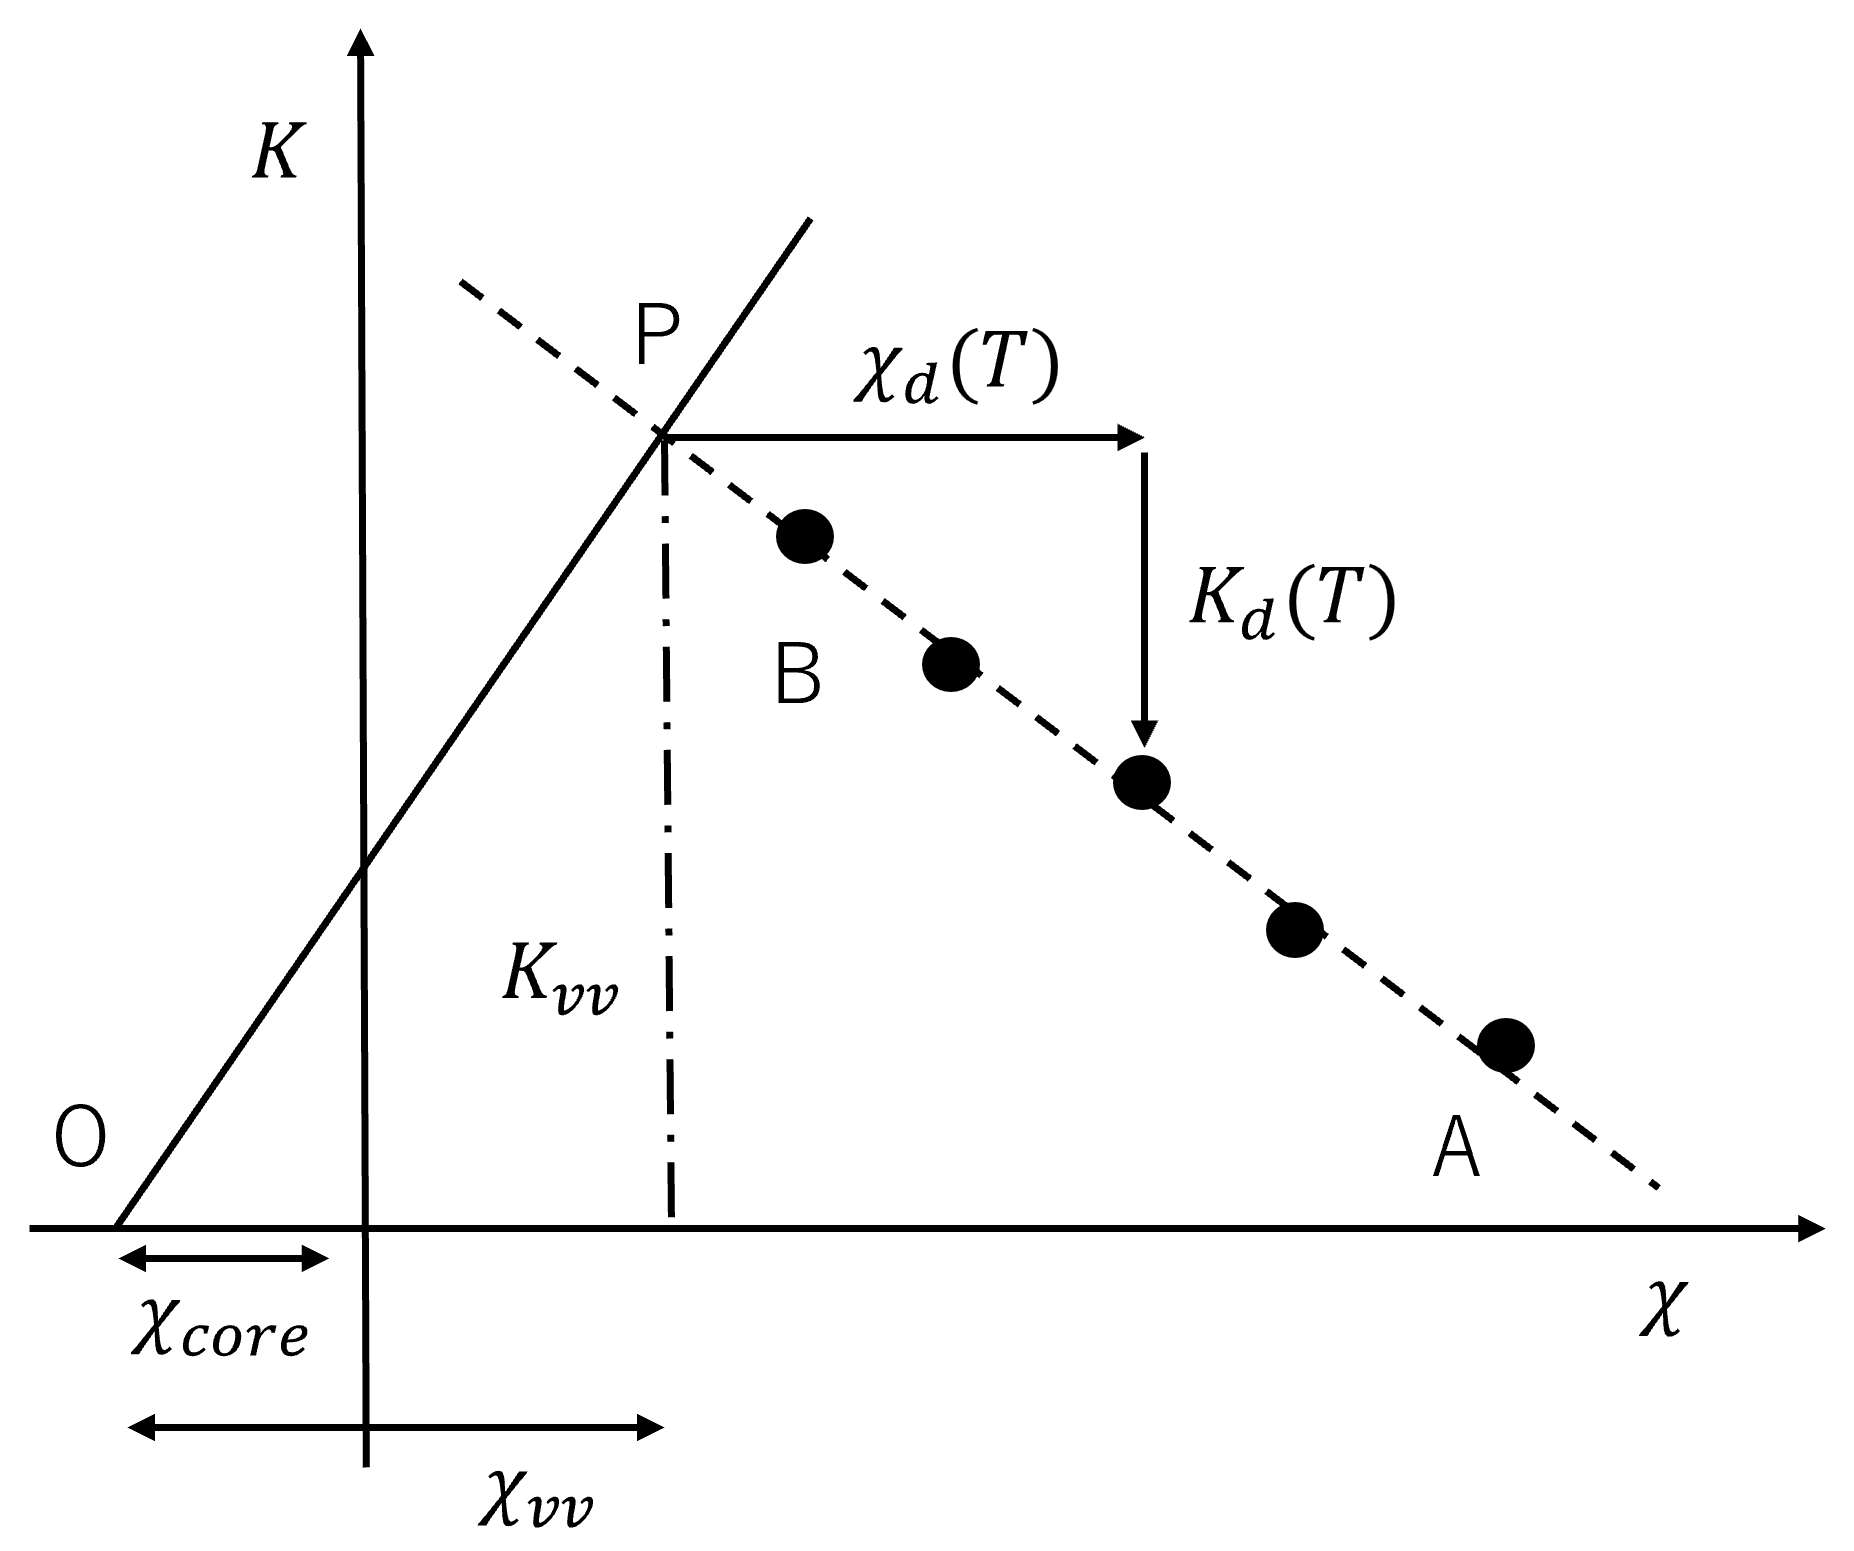
\includegraphics[width=100mm]{./figure/K-X_plot.png}
  \caption{$K-\chi$ plot}
  \label{K-X_plot}
\end{figure}
と書かれる。たとえば、V(バナジウム)金属の$K$は主に$K_{vv}$による、またPd、Ptの負のシフトは$K_d$に起因する。\par
Kや$\chi$が温度変化している場合$\chi_d$が温度変化しているとして、$\chi_d$と$\chi_{\text{vv}}$を分離することができる。各温度における$K$を$\chi$に対してプロットすると実験点は一般に図\ref{K-X_plot}のA-Bのようになる。これを$K-\chi$プロットという。この直線の勾配が$H_{d}^{\text{hf}}$を与える。$\chi_{core}$を使って、原点を0まわりでずらせる。さらに$H_{orb}=2\left\langle1/r^3\right\rangle $を勾配とする直線OPを引き、$K-\chi$プロットの直線との交点Pを求める。このような方法でPd,Ptその他の$K_{\text{vv}},\chi_d$が求められてる。$H_{d}^{\text{hf}}$は波動関数の広がりやs-d混成効果によって敏感に変わるために理論的に評価することは簡単ではないので実験的に求めるしかないが、$\left\langle 1/r^3 \right\rangle$は計算値を使っても大きい誤差はない。

\subsubsection{$f$電子系}
ランタノイド元素やアクチノイド元素を含む$f$電子系希土類化合物では、希土類元素の原子核、たとえば、セリウム(Ce)原子核は、核磁気モーメントを持たず、ウラン(U)原子核は、自然存在比が少なく、核磁気モーメントが小さいためにNMRの観測は難しい。従って、非希土類元素の原子核を対象として、NMRを行う。局在性が強い$f$電子は、周りの構成元素の伝導電子と混成相互作用をしているので、$f$電子のスピン分極や時間的な揺らぎは、伝導電子を媒介にしたトランスファー超微細相互作用を通じて、周りの非希土類元素の核スピンに反映される結果、$f$電子系の情報が得られることになる。\par
$f$電子は、スピンと軌道モーメントの結びつきが強いスピン軌道相互作用(LS相互作用)によって、$d$電子とは異なる特性を示す。このスピン軌道相互作用により、スピン磁気モーメント($S$)と軌道磁気モーメント($L$)は独立ではなく、全角運動量、$J = S + L$によって状態が指定される。この$J$多重項は、さらに結晶場効果によって分裂し、基底状態がクラマース2重項であれば擬スピンを定義できる場合が多い。$f$電子系の特徴は、LS相互作用のために、強い異方性をもち、高温での磁化率は結晶場分裂の大きさと温度の大小関係に依存し、複雑な温度変化を示す。

一方、低温での磁化率は、温度に依存する擬スピン磁化率($\chi_s$)と結晶場励起による温度にあまり依存しないヴァン・ヴレック磁化率($\chi_{\text{vv}}$)からなる。伝導電子による寄与も存在するが、一般的には小さく、$f$電子と伝導電子との混成相互作用を通じてのトランスファー超微細相互作用に起因するナイトシフトが主要な寄与をする。$f$電子系の$\chi_{\text{vv}}$は、
\begin{equation}
  \chi_{\text{vv}, \alpha \beta} = \frac{2 \mu_{\text B}^2}{\hbar} \sum_{n} \frac{\langle 0 | J_{\alpha} | n \rangle \langle n | J_{\beta} | 0 \rangle}{E_n - E_0}
\end{equation}
と表せる。$J = S + L$を考慮すると、$\chi_{\text{vv}}$はスピン成分を含み、$f$原子上での伝導電子とのフント結合を通じて、スピン分極を引き起こす。この分極は、非希土類系原子核の核位置にトランスファーされ、超微細相互作用を通じてナイトシフトに寄与する。

$f$電子系の擬スピン磁化率およびヴァン・ヴレック磁化率によるトランスファー超微細結合定数、$H_s$と$H_{\text{vv}}$は結晶場準位の占有数に依存するので一般に温度変化する。このため、$f$電子系では、$K$-$\chi$プロットによって、両者を分離できない。基底結晶場準位のみで状態を近似できる十分に低温では、非希土類系原子核のナイトシフトは、
\begin{equation}
K = K_s(T) + K_{\text{vv}} + K_c
\end{equation}

\begin{equation}
K_{s, \alpha} = \frac{H_s}{N \mu_{\text B}} \chi_{s, \alpha}
\end{equation}

\begin{equation}
K_{\text{vv}, \alpha} = \frac{H_{\text{vv}}}{N \mu_{\text B}} \chi_{\text{vv}, \alpha}
\end{equation}

として得られる。$H_s$の大きさ、符号、異方性は、分極される伝導電子の軌道波動関数の$s, p, d$対称性によって決まる。$d$対称伝導電子がフェルミ準位に現れない非希土類元素を含む系では、$H_s$は等方的で$f$電子スピン分極1$\mu_{\text B}$あたり数kOeから数十kOe程度、$d$対称伝導電子が現れる系では、マイナス数百kOe程度になる。前者では、最外殻にある$s$対称伝導電子スピンのわずかな分極がフェルミ接触相互作用を通じて、原子核位置に超微細磁場を生む。一方、後者の場合は、$d$対称伝導電子スピンと内殻$s$電子スピンとのフント結合を通じて、外部磁場とは反対方向に分極した内殻$s$電子スピン密度が相対的に大きくなるため符号は負となる。

十分低温では、$\chi_{\text{vv}}$は温度変化しないので$H_{\text{vv}}$の大きさは評価できない。また、伝導電子のスピン、軌道からの寄与は無視できる。結果として、$f$電子系化合物の非希土類元素の原子核の超微細相互作用は、

\begin{equation}
H_{\text{hf}} = \sum_{l} H_{t, l} I \cdot J_l
\end{equation}

と書ける。ここで、$H_{t, l} = H_{s, l} + H_{\text{vv}, l}$、$l$は近接の$f$電子スピンについての和を意味する。

\section{核スピン緩和現象}
\subsection{金属における核磁気緩和率}
スピン格子緩和(縦緩和)は物質内の核スピンが周囲の環境(主に伝導電子など)とエネルギーを交換し、磁化が熱平衡に戻るプロセスを示す。この緩和は核スピンを取り巻く動的な情報を提供し、物質の種類に応じて異なる特性を示す。まず、金属における核スピンと伝導電子との相互作用による$T_1$について考える。$s$バンド電子による緩和はフェルミの接触相互作用
\begin{equation}
  H = -\frac{3\pi}{8} \gamma_e \gamma_n \hbar^2 \delta(r) \left( I_z S_z + \frac{1}{2} \left( I_+ S_- + I_- S_+ \right) \right)
\end{equation}
による。伝導電子はこの相互作用により核スピンとスピンを交換し、運動量を$\hbar\bm k$から$\hbar \bm k'$へと変化させる。この遷移の前後の始状態を$|\psi_i \rangle $、終状態を$|\psi_f\rangle$とすると
\begin{align}
  |\psi_i\rangle &= u_{\bm k}(r)e^{i\bm{k} \cdot \bm{r}} | \downarrow, n \uparrow \rangle = | \bm{k} \downarrow, n \uparrow \rangle, \\
  |\psi_f\rangle &= u_{\bm k'}(r)e^{i\bm{k'} \cdot \bm{r}} | \uparrow, n \downarrow \rangle = | \bm{k'} \uparrow, n \downarrow \rangle
\end{align}
となる。始状態と終状態のエネルギーを$E_i,E_f$とすると、$\hbar(\omega_e-\omega_n)\simeq\omega_e$は非常に小さいので($\omega_e,\omega_n$は電子スピン、核スピンのゼーマン周波数)、遷移確率は
\begin{align}
  W_{\bm k,\bm k'} &\simeq \sum_{\bm{k},\bm{k'}} \frac{2\pi}{\hbar} \left( \frac{8\pi}{3} \gamma_e \gamma_n \hbar^2 \right)^2 \left| \langle \bm k |\delta(\bm r)|\bm k' \rangle \right|^2  \frac{1}{4} \delta(E_{\bm{k}} - E_{\bm{k'}})\\
  &= \int \int \frac{2\pi}{\hbar} \left( \frac{8\pi}{3} \gamma_e \gamma_n \hbar^2 \right)^2 \left| \langle \bm k |\delta(\bm r)| \bm k' \rangle \right|^2 \frac{1}{4} \delta(E_{\bm k} - E_{\bm k'}) \nonumber \\
  &\quad \times N(E_{\bm k}) N(E_{\bm k'}) f(E_{\bm k})(1 - f(E_{\bm k'})) \, dE_{\bm k} \, dE_{\bm k'}
\end{align}
となる。ここで、$N(E_{\bm{k}})$,$f(E_{\bm{k'}})$は状態密度とフェルミ関数である。また
\begin{equation}
  f(E_{\bm k})(1 - f(E_{\bm k})) \simeq -k_{\text B} T \frac{\partial f(E_{\bm k})}{\partial E_{\bm k}}\simeq k_{\text B} T \, \delta(E - E_F)
\end{equation}
であるから
\begin{equation}
  \frac{1}{T_1}=2W=\frac{64}{9}\pi^3\gamma^2_e\gamma^2_n\hbar^3|u_{k_F}(0)|^4N^2(E_F)k_{\text B}T
  \label{T1metal}
\end{equation}
となり、$1/T_1$は$T$に比例する。ここで、式(\ref{K_s_3})と式(\ref{T1metal})から、$T_1$と$K_s$の関係
\begin{equation}
  T_1TK^2_s=\frac{\hbar}{4\pi k_{\text B}}\left(\frac{\gamma_e}{\gamma_n}\right)^2
\end{equation}
が得られる。これをコリンハの関係式という。\par
式(\ref{K_s_N})のように$s$電子1個あたりの超微細磁場$H^s_{hf}$を用いると、式(\ref{T1metal})は
\begin{equation}
  \left(\frac{1}{T_1}\right)_F = \frac{4\pi}{\hbar}(\gamma_n\hbar H^s_hf)^2\frac{N^2(E_F)}{N^2}k_{\text B}T
\end{equation}
ともかける。これは$s$電子のフェルミの接触相互作用による$T_1$である。

\subsection{核磁気緩和率一般的表示}
磁性体、超電導物資、強相関で物質の構成元素の非磁性原子、磁性原子の核スピン系と電子スピン系は、ほとんどの場合スカラー型の磁気的相互作用をしており、全ハミルトニアンは、
\begin{equation}
 \mathcal H_{IS} = -\gamma_n\hbar I_z\cdot H_z + \sum_l H_{s,l} \left(I_z S_{lz}+\frac{1}{2}\left\{I_+ S_{l-}(t)+I_-S_{l+}(t)\right\}\right) + \mathcal H_e
\end{equation}
と書ける。ここで、各項は次の要素からなる。
\begin{itemize}
  \item 第一項: $-\gamma_n \hbar I_z \cdot H_z$\\
  核スピン $I_z$ が外部磁場 $H_z$ と相互作用するゼーマンエネルギー
  \item 第二項: $H_{s,l} I_z S_{lz}$\\
  核スピン $I_z$ と電子スピン $S_{lz}$ のz方向成分の相互作用(長距離相互作用成分も含む)
  \item 第三項: $\frac{1}{2} \left\{ I_+ S_{l-}(t) + I_- S_{l+}(t) \right\}$\\
  スピンと電子スピンが相互に状態を交換する、いわゆる「スピンフリップフロップ」過程を表す。
  \item 第四項: $\mathcal H_e$\\
  他の環境や結晶場との相互作用を含むエネルギー項
\end{itemize}
時間に依存する摂動、$\mathcal H'_{IS}(t) = (H_{s,l}/2)\left\{I_+S_{l-}+I_-S_{l+}\right\}$による核スピンレベル、$I_z=|m\rangle,|m+1\rangle $間の遷移確率は、電子スピン系の固有状態、$|M\rangle,|M'\rangle$のエネルギー保存則、$\hbar \omega_n = E_M - E_{M'}$を満たす遷移を伴って、
\begin{equation}
  W_{m\rightarrow m+1} = \frac{2\pi}{\hbar} \sum_{M,M'}P_M|\langle m+1,M'|\mathcal H'_{IS}(t)|m,M\rangle|^2 \delta(E_M-E_{M'}-\hbar \omega_n) 
\end{equation}
で与えられる。ここで、$\omega_n$は核スピン系ゼーマン周波数、$P_M$は電子スピン系の固有状態$|M\rangle$の温度$T$における統計分布確率である。
\begin{equation}
  \delta(x) = \frac{1}{2\pi} \int_{-\infty}^{\infty} e^{i x t} \, dt
\end{equation}
を使って変形すると
\begin{equation}
  W_{m \rightarrow m+1} = \frac{H_{s,l, \perp}^2}{4} (I - m)(I + m + 1) \sum_{M, l} P_M \left\langle M \left| S_{l+}(t)S_{l-}(0) \right| M \right\rangle e^{-i \hbar \omega_n t} \, dt
\end{equation}
が得られる。
\begin{equation}
  \frac{1}{T_1}=\frac{W_{m \rightarrow m+1}+W_{m+1\rightarrow m}}{(I-m)(I+m+1)}
\end{equation}
であるから、$T_1$ は
\begin{equation}
  \frac{1}{T_1} = \sum_{l}\frac{H^2_{s,l,\bot}}{4}\int_{-\infty}^{\infty} \langle S_l^+(t) S_l^-(0) + S_l^-(t) S_l^+(0) \rangle e^{-i \hbar \omega_n t} \,dt
\end{equation}
を得る。ここで$[A,B]=(AB+BA)/2$を使って、まとめると
\begin{equation}
  \frac{1}{T_1} = \frac{1}{2} \sum_l H_{s,l, \perp}^2 \int_{-\infty}^{\infty} \langle [S_{l+}(t), S_{l-}(0)] \rangle e^{-i \hbar \omega_n t} \, dt
\end{equation}
このように,$1/T_1$は電子スピンのゆらぎの時間相関関数のフーリエ周波数スペクトルの成分の中で,NMR周波数 $\omega_n$ でのスペクトル密度に比例している。さらに,$ \bm{S}(\bm q) = \sum_l \bm{S}_l e^{i \bm q \cdot \bm {r_l}}$ とフーリエ展開すると,
\begin{equation}
\frac{1}{T_1} = \frac{1}{2} \sum_{\bm q} (\bm H_{\bm q} \bm H_{-\bm {q}})_{\perp} \int_{-\infty}^{\infty} \langle [S_+(-\bm {q}, t), S_-(\bm {q}, 0)] \rangle e^{-i \hbar \omega_n t} \, dt
\end{equation}
常磁性状態では揺動散逸定理により,
\begin{equation}
  \frac{1}{2} \int_{-\infty}^{\infty} \langle [S_+(-\bm {q}, t), S_-(\bm q, 0)] \rangle e^{-i \hbar \omega_n t} \, dt = \frac{2 \chi''_{\perp}(\bm q, \omega_n)}{(2\mu_{\text B})^2(1 - e^{-\hbar \omega_n / k_{\text B} T})}
\end{equation}
に従う。ここで、$\hbar\omega_n\ll k_{\text B}T$を考慮すると
\begin{equation}
\frac{1}{T_1} = \frac{2 k_{\text B} T}{\hbar (2 \mu_{\text B})^2} \sum_{\bm q} (\bm H_{\bm q} \bm H_{-\bm {q}})_{\perp} \frac{\chi''_{\perp}(\bm q, \omega_n)}{\omega_n}
\label{T1_a}
\end{equation}
$ \chi''_{\perp}(\bm q, \omega) $ は波数 $ \bm q $ および角周波数 $ \omega $ に依存する動的磁化率の虚数部であり、$\sum _{\bm q}\chi''_{\perp}(\bm q, \omega)$から全波数の和となることがわかる。また、$\bot$はNMR/NQRでの磁場および、電場勾配の主軸、すなわち核スピン系の量子化軸に対して垂直な成分を表している。通常金属の場合、動的帯磁率は、
フェルミ分布関数 $ f(\varepsilon) $ を用いると
\begin{equation}
\chi_0(\bm q, \omega) = (2\mu_{\text B})^2 \sum_{\bm k} \frac{f(\varepsilon_{\bm k+\bm q}) - f(\varepsilon_{\bm k})}{\hbar \omega - (\varepsilon_{\bm k+\bm q} - \varepsilon_{\bm k}) + i \Gamma}
\end{equation}
となる。ここで$\chi_0(\bm q, \omega)=\chi'_0(\bm q,\omega)-i\chi''_0(\bm q,\omega)$であるから
\begin{align}
  \chi''_0(\bm q,\omega) &= (2\mu_{\text B})^2\pi \sum_{\bm K}{\delta(\varepsilon_{\bm k}-\varepsilon_{\bm{k+q}}-\hbar\omega)[f(\varepsilon_{\bm{k+q}})-f(\varepsilon_{\bm k})]}\\
  &=(2\mu_{\text B})^2\pi\int d\varepsilon N(\varepsilon)\delta(\varepsilon-\varepsilon'-\hbar\omega)[f(\varepsilon')-f(\varepsilon)]\,\\
  &= (2\mu_{\text B})^2 \pi N(\varepsilon'+\hbar\omega)(\hbar\omega)\left(-\frac{\partial f}{\partial \varepsilon'}\right)
\end{align}
\begin{align}
  \sum_{\bm q} \chi''_\bot(\bm q,\omega) &= (2\mu_{\text B})^2 \pi \int d\varepsilon' N(\varepsilon')N(\varepsilon'+\hbar\omega)(\hbar\omega)\delta(\varepsilon'-E_{\text F})\\
  &= (2\mu_{\text B})^2\pi(\hbar\omega)N(E_{\text F})^2
  \label{sum_chi_img}
\end{align}
となる。超微細相互作用係数$ A(r) $ は空間的に局在し$ \delta $関数であらわせるので、この関数の波数空間へのフーリエ変換は
\begin{equation}
  A(\bm q)=\int_{-\infty}^{\infty} A(\bm r)e^{-i \bm q \cdot r}\,d \bm r = e^{-i \bm q \cdot 0}=1
\end{equation}
となる。したがって、$A(\bm q)$は波数$\bm q$に依存しないので定数として扱える。そのためフーリエ変換された超微細相互作用の強さ$H_q$の平方のうち、核スピンの量子化軸(つまり外部磁場方向や電場勾配方向)に対して垂直な成分$(H_{\bm q}H_{-\bm q})_\bot$は定数$A^2$と表せる。よって式 (\ref{T1_a}) に式 (\ref{sum_chi_img}) をいれると,
\begin{equation}
  \frac{1}{T_1} \propto A^2 N(E_{\text F})^2 k_{\text B} T
\end{equation}
と書ける。ナイト・シフトにおける

磁性体,電子相関効果で磁性が発現する遍歴電子系や新奇な超伝導を含む多彩な電子状態が観測される強相関物質では,スピンの揺らぎ効果によって,$\chi(q,\omega)$ は,特徴的な波数および周波数変化を示し,緩和現象に際立った特徴をもたらす.図3.7には,通常金属の $\chi_0(q,\omega)$ および,波数依存するスピン揺らぎが顕著な場合の,$\chi(Q+q,\omega)$ を示す.前者の場合,$\chi_0(q,\omega)$ はエネルギー $\omega$ に比例し,その傾きは $N(E_F)$ で与えられる.後者の場合は,



\begin{equation}
  \chi(Q+q,\omega) \propto \frac{\omega \Gamma_{Q+q}}{\omega^2 + \Gamma_{Q+q}^2} 
\end{equation}


\chapter{電気四重極相互作用}
本研究では、1/1近似結晶Au$_{71}$Al$_{15}$Tb$_{14}$のAlに対してNMRを行っているが、Alは$I=5/2$である。原子核は$I \geq 1$の場合、磁気モーメントに加えて電気四重極能率(モーメント)を持つ。これと周辺の電荷が作る電場勾配との相互作用は、核スピンのエネルギー状態を分裂させ、外部磁場をかけなくとも核四重極共鳴(NQR)を可能にし、NMRにさらに多彩な変化をもたらす。本章では、この相互作用によって生じる効果について述べる。

\section{核四重極共鳴(NQR)}
原子核は$I \geq 1$の場合、磁気モーメントに加えて電気四重極能率$eQ$を持つ。ここで$e$は陽子の電荷である。これは、原子核の形が回転楕円体になっていることから生じるもので、電気四重極能率は
\begin{equation}
  eQ = e \int_V (3z^2 - r^2) dv
\end{equation}
と定義される。$z$は回転軸、すなわちスピンの方向であり、$V$は原子核の体積である。回転軸が楕円体の長軸ならば$Q > 0$、短軸ならば$Q < 0$となる。

原子核の近傍に電荷があると、楕円体の原子核ではその向きによってクーロンエネルギーに違いが生じる。すなわち、磁場を印加しなくてもスピンの縮退が解け、この分離したエネルギー間隔に等しい振動磁場を量子化軸に垂直に加えると遷移が起こる。これを、核四重極共鳴(NQR)という。

\section{電気四重極ハミルトニアン}
原子核内の陽子の密度を$\rho(\mathbf{r})$、核外の電荷(電子または当該イオンの外部にあるイオン)による静電ポテンシャルを$V(\mathbf{r})$とすると、クーロンエネルギーは
\begin{equation}
  E = \int \rho(\mathbf{r}) V(\mathbf{r}) dv
  \label{q_en}
\end{equation}
である。核の大きさは電子の広がりより十分小さいので、$V(r)$を原点周りで展開すると
\begin{equation}
V(\mathbf{r}) = V(0) + \sum_i x_i \frac{\partial V}{\partial x_i}\Big|_{r=0} + \frac{1}{2} \sum_{i,j} x_i x_j \frac{\partial^2 V}{\partial x_i \partial x_j}\Big|_{r=0} + \cdots
\end{equation}
となり、これを式(\ref{q_en})に入れると
\begin{equation}
  E = V(0) \int \rho(\mathbf{r}) dv + \sum_i V_i \int x_i \rho(\mathbf{r}) dv + \frac{1}{2} \sum_{i,j} V_{ij} \int x_i x_j \rho(\mathbf{r}) dv + \cdots
  \label{e_tenkai}
\end{equation}
ここで、$x, y, z = x_1, x_2, x_3$であり、$V_i = \partial V/\partial x_i$、$V_{ij} = \partial^2 V/\partial x_i \partial x_j$である。
式(\ref{e_tenkai})の第1項は一定値であり、回転楕円体は電気双極子能率を持たないことから第2項は0となる。よって第三項が電気四重極相互作用である。ここで、電気四重極テンソル
\begin{equation}
  Q_{ij} = \int (3 x_i x_j - \delta_{ij} r^2) \rho(\mathbf{r}) dv
\end{equation}
を導入して
\begin{equation}
  \int x_i x_j \rho(\mathbf{r}) \, dv = \frac{1}{3} \left[ Q_{ij} + \delta_{ij} \int r^2 \rho(\mathbf{r}) \, dv \right]
  \label{xxij}
\end{equation}
と書き直す。これを式(\ref{e_tenkai})に代入するが、ここで式(\ref{xxjj})の第2項は、核外電荷による$V(\bm r)$はラプラスの方程式
\begin{equation}
  \Delta V = \sum_{i,j}V_{ij}\sigma_{ij}=0
\end{equation}
を満たす。よって、式(\ref{e_tenkai})の第3項は
\begin{equation}
  \mathcal{H}_Q = \frac{1}{6}\sum_{i,j}V_{ij}Q_{ij}
\end{equation}
とかける。さらに、核内の$k$番目の用紙の位置を$\bm {r}_k$とフーリエ展開すると
\begin{equation}
  \rho(\bm r)=e\sum_K\sigma(\bm r- \bm {r}_k)
\end{equation}


\chapter{A.C.磁化率測定の原理}
\section{線形応答理論}
線形応答理論は、物理系が外部からの小さな摂動(外場)に対してどのように応答するかを記述する理論である。線形応答理論は以下の二つを前提とする。
\begin{enumerate}[label=\textnormal{(\Roman*)}]
  \item 入力が$a$倍されると、応答も単に$a$倍される。
  \item 複数の入力に対する応答は、各入力に対する応答の和で表される。
\end{enumerate}
また、外場の影響で生じる物理量の変化が、外場に対して線形に依存するのは
\begin{equation}
  A(F)=A(0)+A'(0)F+O(F^2)
\end{equation}
などと物理量をパラメータ展開した時に、2次以降の項が十分無視できる、$F$が十分小さい時である。\par
あるデルタ関数的な入力に対する応答を$\chi(t)$として、動的な外場$F(t)$をゆっくりと加えた時の応答を考える。前提(I)より応答$\chi(t)$は入力$F(t')$に比例して大きくなるので、
\begin{equation}
  F(t')\cdot\chi(t-t')
\end{equation}
また、前提($\textsc{ii}$)よりある時刻$t$における物理量$A(t)$は
\begin{equation}
 A(t)=A(t_0)+\int_{-\infty}^{t}{dt'F(t') \chi(t-t')}
 \label{A(t)}
\end{equation}
と表せる。ここで式(\ref{A(t)})の第二項は、畳み込み積分とよばれ、ある時刻$t$における応答が過去の入力に対してどのように影響されるかを表す。
\begin{figure}[htbp]
  \centering
  \vspace{10mm}
  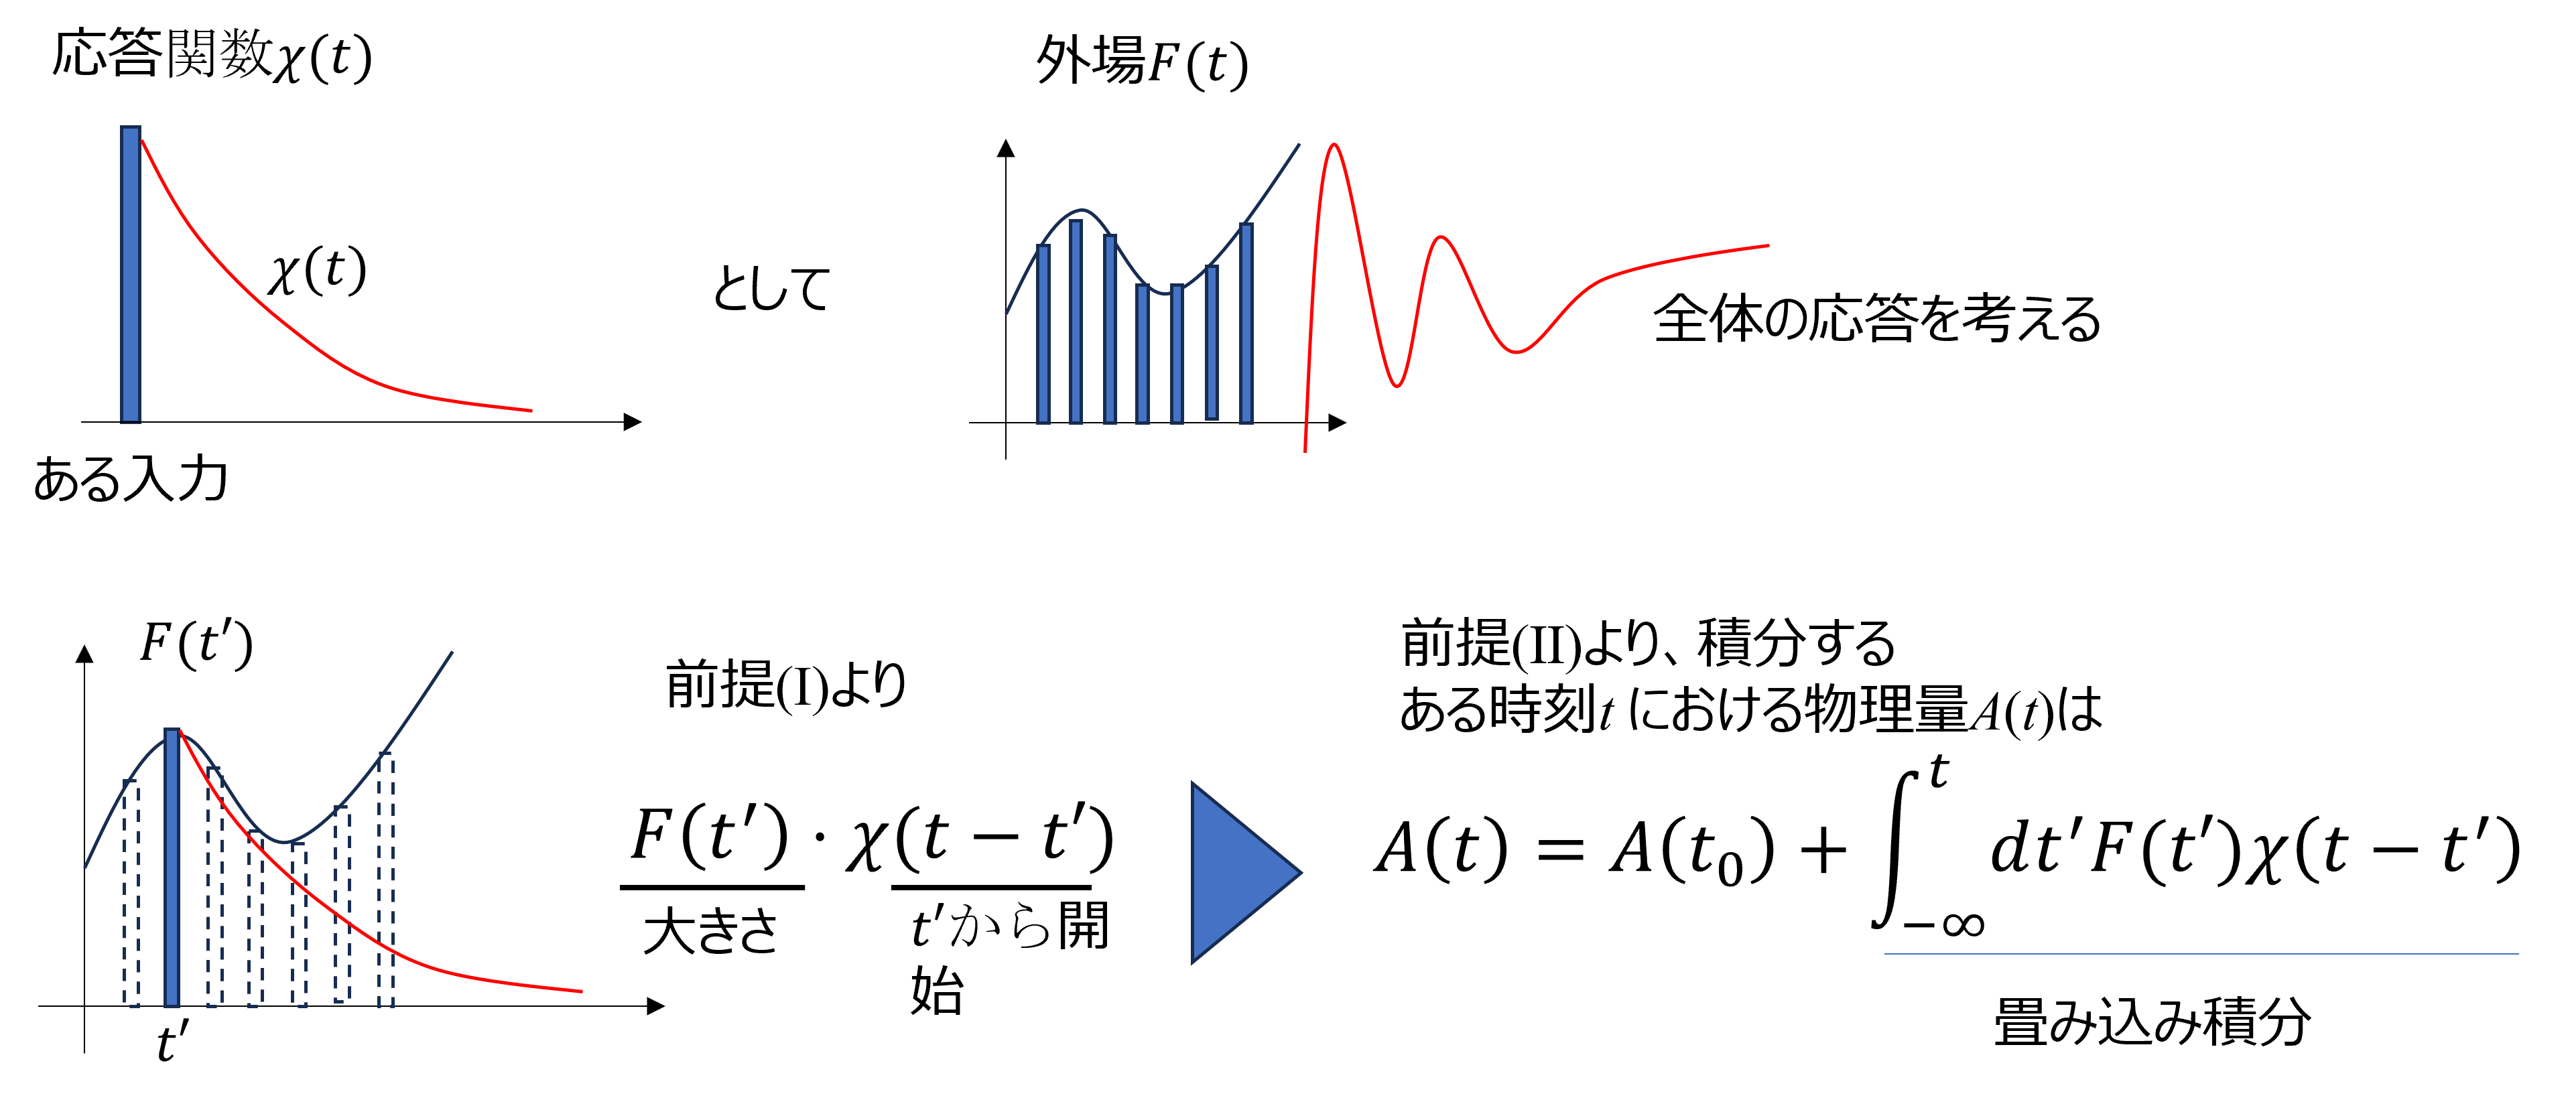
\includegraphics[width=160mm]{./figure/liner_theory.png}
  \caption{線形応答理論}
  \label{liner_theroy}
\end{figure}

また、応答が未来の原因から影響を受けないようにすることで、時間方向の矛盾を避け、物理系の時間対称性を保証すること(因果律)を考慮すると応答関数$\chi(t)$は
\begin{align}
  \chi^R(t'') &= \chi(t'')\theta(t'') \label{chi_R} \\
  \theta(t'') &= \begin{cases} 
     1 & (t'' > 0)  \\
     0 & (t'' < 0)
   \end{cases} \label{theta_w}
 \end{align}
と変換される。これを用いると、式(\ref{A(t)})は
\begin{equation}
  A(t)=A(t_0)+\int_{-\infty}^{\infty}{dt'F(t') \chi^R(t-t')}
\end{equation}
となる。$A(t)$をフーリエ変換$A(\omega)$を求める。
\begin{equation}
  A(\omega)=\int_{-\infty}^{\infty} \left( \int_{-\infty}^{\infty} F(t') \chi^R(t - t') \, dt' \right) e^{i \omega t} \, dt
\end{equation}
ここで積分の順序を入れ替えると
\begin{equation}
  A(\omega) = \int_{-\infty}^{\infty} F(t') \left( \int_{-\infty}^{\infty} \chi^R(t - t') e^{i \omega t} \, dt \right) dt'
\end{equation}
ここで、$\tau=t-t'$の置換を行うと、$t=\tau+t',dt=d\tau$であるから
\begin{equation}
  A(\omega) = \int_{-\infty}^{\infty} F(t') \left( \int_{-\infty}^{\infty} \chi^R(\tau) e^{i \omega (\tau + t')} \, d\tau \right) dt'
\end{equation}

積分の中で $e^{i \omega (\tau + t')}$ を分離すると、
\begin{equation}
  A(\omega)= \int_{-\infty}^{\infty} F(t') e^{i \omega t'} \left( \int_{-\infty}^{\infty} \chi^R(\tau) e^{i \omega \tau} \, d\tau \right) dt'
\end{equation}
となる。ここで、フーリエ変換の定義式から
\begin{equation}
  \int_{-\infty}^{\infty} F(t') e^{i \omega t'} \, dt' = \tilde{F}(\omega)
\end{equation}
\begin{equation}
  \int_{-\infty}^{\infty} \chi^R(\tau) e^{i \omega \tau} \, d\tau = \tilde{\chi}^R(\omega)
\end{equation}
したがって、$A(t)$のフーリエ変換$A(\omega)$は
\begin{equation}
  A(\omega)= \tilde{F}(\omega) \tilde{\chi}^R(\omega)
\end{equation}
となる。ここで$\tilde{\chi}^R(\omega)$は感受率を表す。\par
また、階段関数$\theta(t)$ のフーリエ変換は式(\ref{theta_w})からわかる通り、$t>0$においては$0$なので
\begin{equation}
  \tilde{\theta}(\omega) = \int_{0}^{\infty} e^{i \omega t} \, dt = \left[ \frac{e^{i \omega t}}{i \omega} \right]_{0}^{\infty}
\end{equation}
となる。
このままだと$t \to \infty$で収束しないため、収束を保証するために $\omega$ に小さな虚数部分 $i \eta(\eta \to 0^+)$ を加える。したがって、
\begin{equation}
  \tilde{\theta}(\omega) = \int_{0}^{\infty} e^{i (\omega + i \eta) t} \, dt = \left[ \frac{e^{i (\omega + i \eta) t}}{i (\omega + i \eta)} \right]_{0}^{\infty}
\end{equation}
となり、これを評価すると、
\begin{equation}
  \tilde{\theta}(\omega) = \lim_{\eta \to 0^+} \frac{1}{i (\omega + i \eta)}
\end{equation}
となる。さらに、分母の虚数成分を分離し、デルタ関数の定義 $\delta(\omega) = \lim_{\eta \to 0^+} \frac{\eta}{\pi (\omega^2 + \eta^2)}$ を用いると、
\begin{align}
  \tilde{\theta}(\omega) &= \lim_{\eta \to 0^+} \left( \frac{\omega}{\omega^2 + \eta^2} - i \frac{\eta}{\omega^2 + \eta^2} \right)\\
  &= \pi \delta(\omega) - \frac{i}{\omega}
  \label{theta_omega1}
\end{align}
となるa。\par
ここで、周波数領域での畳み込み積分は$\tilde{\theta}(\omega)$をもちいて
\begin{equation}
  \chi^R(\omega) = \frac{1}{2\pi}\int_{-\infty}^{\infty} \tilde{\theta}(\omega - \omega') \cdot \chi(\omega') \, d\omega'
\end{equation}
と表される。式(\ref{theta_omega1})を代入すると
\begin{equation}
  \chi^R(\omega) = \frac{1}{2\pi} \int_{-\infty}^{\infty} \left[ \pi \delta(\omega - \omega') - \frac{i}{(\omega - \omega')} \right]\chi(\omega') \, d\omega'
\end{equation}
ここで、デルタ関数の性質より
\begin{equation}
  \int_{-\infty}^{\infty} \delta(\omega - \omega') f(\omega') \, d\omega' = f(\omega)
\end{equation}
したがって、
\begin{equation}
  \frac{1}{2\pi} \cdot \pi \delta(\omega - \omega') \chi(\omega') = \frac{1}{2} \chi(\omega)
\end{equation}
また特異点を持つ項$-\frac{i}{\omega-\omega'}$は主値積分として扱い
\begin{equation}
  -\frac{i}{2\pi} \int_{-\infty}^{\infty} \frac{\chi(\omega')}{\omega - \omega'} \, d\omega' = -\frac{i}{2\pi} \, P\int_{-\infty}^{\infty} \frac{\chi(\omega')}{\omega - \omega'} \, d\omega'
\end{equation}
以上をまとめると
\begin{equation}
  \chi^R(\omega) = \frac{1}{2} \chi(\omega) - \frac{i}{2\pi} \, P \int_{-\infty}^{\infty} \frac{\chi(\omega')}{\omega' - \omega} \, d\omega'=\chi'(\omega)+i\chi''(\omega)
\end{equation}
となる。ここで、実部と虚部の関数$\chi'(\omega),\chi''(\omega)$はクラマース・クロニッヒの定理で結ばれる。
\section{久保公式による応答関数の導出}
時間依存のハミルトニアンを以下のように定義する。
\begin{equation}
  H(t) = H_0 - A F(t)
\end{equation}
ここで、密度行列 $\rho(t)$ の時間発展は、シュレディンガー方程式に従うので
\begin{equation}
  i\hbar \frac{d \rho(t)}{dt} = [H(t), \rho(t)] 
\end{equation}
さらに時間 $t = -\infty$ では、系は熱平衡状態にあるので
\begin{equation}
  \rho(-\infty) = \frac{1}{Z_0} e^{-\beta H_0} = \rho_0 
\end{equation}
ここで、$ Z_0 $ は分配関数、$ \beta = \dfrac{1}{k_{\text B} T} $ は逆温度である。\par
外部場は断熱的にスイッチオンされるので
\begin{equation}
  F(t) = e^{s t} f(t), \quad s \rightarrow +0 
\end{equation}
ここで、$ s $ は正の無限小量であり、断熱的な導入を表現している。\par
密度行列を摂動展開すると
\begin{equation}
  \rho(t) = \rho_0 + \rho_1(t) + O(F^2) 
\end{equation}
ここで、$ \rho_1(t)$ は外部場に対する一次の応答を表す。
一次の項を取り出して、式 () に代入すると  
\begin{equation}
  i\hbar \frac{d \rho_1(t)}{dt} = [H_0 - A F(t), \rho_0 + \rho_1(t)]
\end{equation}
摂動の一次まで考慮し、二次以上の項を無視すると  
\begin{equation}
  i\hbar \frac{d \rho_1(t)}{dt} - [H_0, \rho_1(t)] = - F(t) [A, \rho_0] 
\end{equation}
 相互作用描像における密度行列を次のように定義する。
\begin{equation}
  \rho_1(t) = e^{-i H_0 t / \hbar} \tilde{\rho}_1(t) e^{i H_0 t / \hbar}
\end{equation}
これを式 () に代入すると、方程式は
\begin{equation}
  i\hbar \frac{d \tilde{\rho}_1(t)}{dt} = - F(t) e^{i H_0 t / \hbar} [A, \rho_0] e^{-i H_0 t / \hbar} \label{eq:3.8}
\end{equation}
となる。両辺を時間 $ t' $ で積分すると
\begin{equation}
  \tilde{\rho}_1(t) = \frac{i}{\hbar} \int_{-\infty}^{t} dt' \, e^{i H_0 t' / \hbar} [A, \rho_0] e^{-i H_0 t' / \hbar} F(t') \label{eq:3.9}
\end{equation}
元の描像に戻すと
\begin{equation}
  \begin{aligned}
    \rho_1(t) &= e^{-i H_0 t / \hbar} \tilde{\rho}_1(t) e^{i H_0 t / \hbar} \\
    &= \frac{i}{\hbar} \int_{-\infty}^{t} dt' \, e^{-i H_0 (t - t') / \hbar} [A, \rho_0] e^{i H_0 (t - t') / \hbar} F(t') \label{eq:3.10}
  \end{aligned}
\end{equation}
物理量 $ B $ の期待値は  
\begin{equation}
  \langle B \rangle_t = \mathrm{Tr}[\rho(t) B] \approx \mathrm{Tr}[\rho_1(t) B]
\end{equation}
これを計算すると
\begin{equation}
  \langle B \rangle_t = \frac{i}{\hbar} \int_{-\infty}^{t} dt' \, \mathrm{Tr}\left( e^{-i H_0 (t - t') / \hbar} [A, \rho_0] e^{i H_0 (t - t') / \hbar} B \right) F(t')
\end{equation}
ハミルトニアン $H_0$ に関する演算子の時間依存性を用いて、$A(t) = e^{i H_0 t / \hbar} A e^{-i H_0 t / \hbar}$ と表せるので 
\begin{equation}
  \langle B \rangle_t = \frac{i}{\hbar} \int_{-\infty}^{t} dt' \, \mathrm{Tr}\left( [A(t' - t), \rho_0] B \right) F(t') 
\end{equation}
さらに、トレースの性質と交換子の循環性を利用すると
\begin{equation}
  \langle B \rangle_t = \frac{i}{\hbar} \int_{-\infty}^{t} dt' \, \mathrm{Tr}\left( \rho_0 [B, A(t - t')] \right) F(t') 
\end{equation}
という形になる。よって応答関数は
\begin{equation}
  K_{BA}(t - t') = \frac{i}{\hbar} \mathrm{Tr}\left( \rho_0 [B, A(t - t')] \right)
\end{equation}
である。
\section{線形応答理論の具体例-減衰調和振動子}
図のようなばねに繋がれた物体が摩擦のある面を振動する時を考える。\par
この系の運動方程式は
\begin{equation}
  F=\left(m\left(\frac{d}{dt}\right)^2+\alpha\frac{d}{dt}+K\right)
\end{equation}
この運動方程式をフーリエ変換すると
\begin{equation}
 F(\omega)=(-m\omega^2+i\alpha\omega+k)\chi(\omega)
\end{equation}
共鳴周波数$\omega_0^2=k/m$、摩擦係数$\gamma=\alpha/m$を用いると
\begin{equation}
  F(\omega)=m(\omega_0^2-\omega^2-i\omega\gamma)\chi(\omega)
\end{equation}
となる。よって、感受率は
\begin{equation}
 \chi^R(\omega)=\frac{A(\omega)}{F(\omega)}=\frac{1}{m(\omega_0^2-\omega^2-i\omega\gamma)}=\frac{(\omega_0^2 - \omega^2)/m}
 {\left(\omega_0^2 - \omega^2\right)^2 + \left(\omega \gamma\right)^2} + i \frac{\omega \gamma / m}{\left(\omega_0^2 - \omega^2\right)^2 + \left(\omega \gamma\right)^2}
\end{equation}
となる。
\section{磁化率の場合}
磁化率Mの外場に対する応答を考える。磁化$M$が外場$H$に対してどのように応答するのかを記述する微分方程式は
\begin{equation}
 \alpha\dot{M}+kM=H
 \label{f}
\end{equation}
で表される。ここで、第一項は磁化の減衰をあらわす項であり、第二項は磁化の復元力を表す。
また$f=0$を考えると
\begin{equation}
  M(t)=M(0)e^{-t/\tau}
\end{equation}
が得られる。つまり、システムが磁化を持ち、その磁化が時間とともに指数関数的に緩和する場合、式(\ref{f})として考えることができる。
この微分方程式から得られる感受率は
\begin{equation}
  \chi_M^R = \frac{1/k}{1-i\omega\tau}
\end{equation}
である。ここで$\tau= \frac{\alpha}{k}$は緩和時間をあらわす。また、断熱磁化率$\chi_S$を追加すると
\begin{equation}
  \chi_M^R = \chi_S+\frac{1/k}{1-i\omega\tau} 
\end{equation}
となる。さらに、等温磁化率$\chi_T=\chi_S+1/k$として、実部と虚部に分けると
\begin{equation}
  \chi_M^R=\chi_S+\frac{\chi_T-\chi_S}{1+\omega^2\tau^2}+i\frac{\chi_T-\chi_S}{1+\omega^2\tau^2}\omega\tau
  \label{outoukanss}
\end{equation}
となる。よって式(\ref{outoukanss})より、磁気モーメントの緩和時間$\tau$に応じて、周波数$\omega$と$1/\tau$の相対的な大きさに基づいて、以下の三つの領域が定義される。
\begin{itemize}
  \item $\omega\ll 1/\tau$\par
  この領域は、交流磁場に対して系がほぼ即時に応答する直流($d.c.$)限界に対応し、直流磁化率が得られる。これは、平衡応答であり、磁気モーメントが格子とエネルギーを交換できる状態である。その結果、等温応答磁化率$\chi_T$が測定される。
  \item $\omega\gg 1/\tau$\par
  この領域は、系の磁気モーメントが応答するには振動磁場が早すぎる場合である。したがって、系は格子とエネルギーを交換する時間がないので、この時得られる磁化率は、断熱磁化率$\chi_S$が測定される。
  \item $\omega\approx 1/\tau$\par
  この中間の領域では、交流磁場の周波数が系の磁気緩和の時間スケールと比較可能であり、より複雑な応答が得られる。また、応答は実部と虚部の成分$\chi'_{a.c.}$および$\chi''_{a.c.}$からなり、周波数依存性は図\ref{outou}のようになる。
\end{itemize}
\begin{figure}[htbp]
  \centering
  \vspace{10mm}
  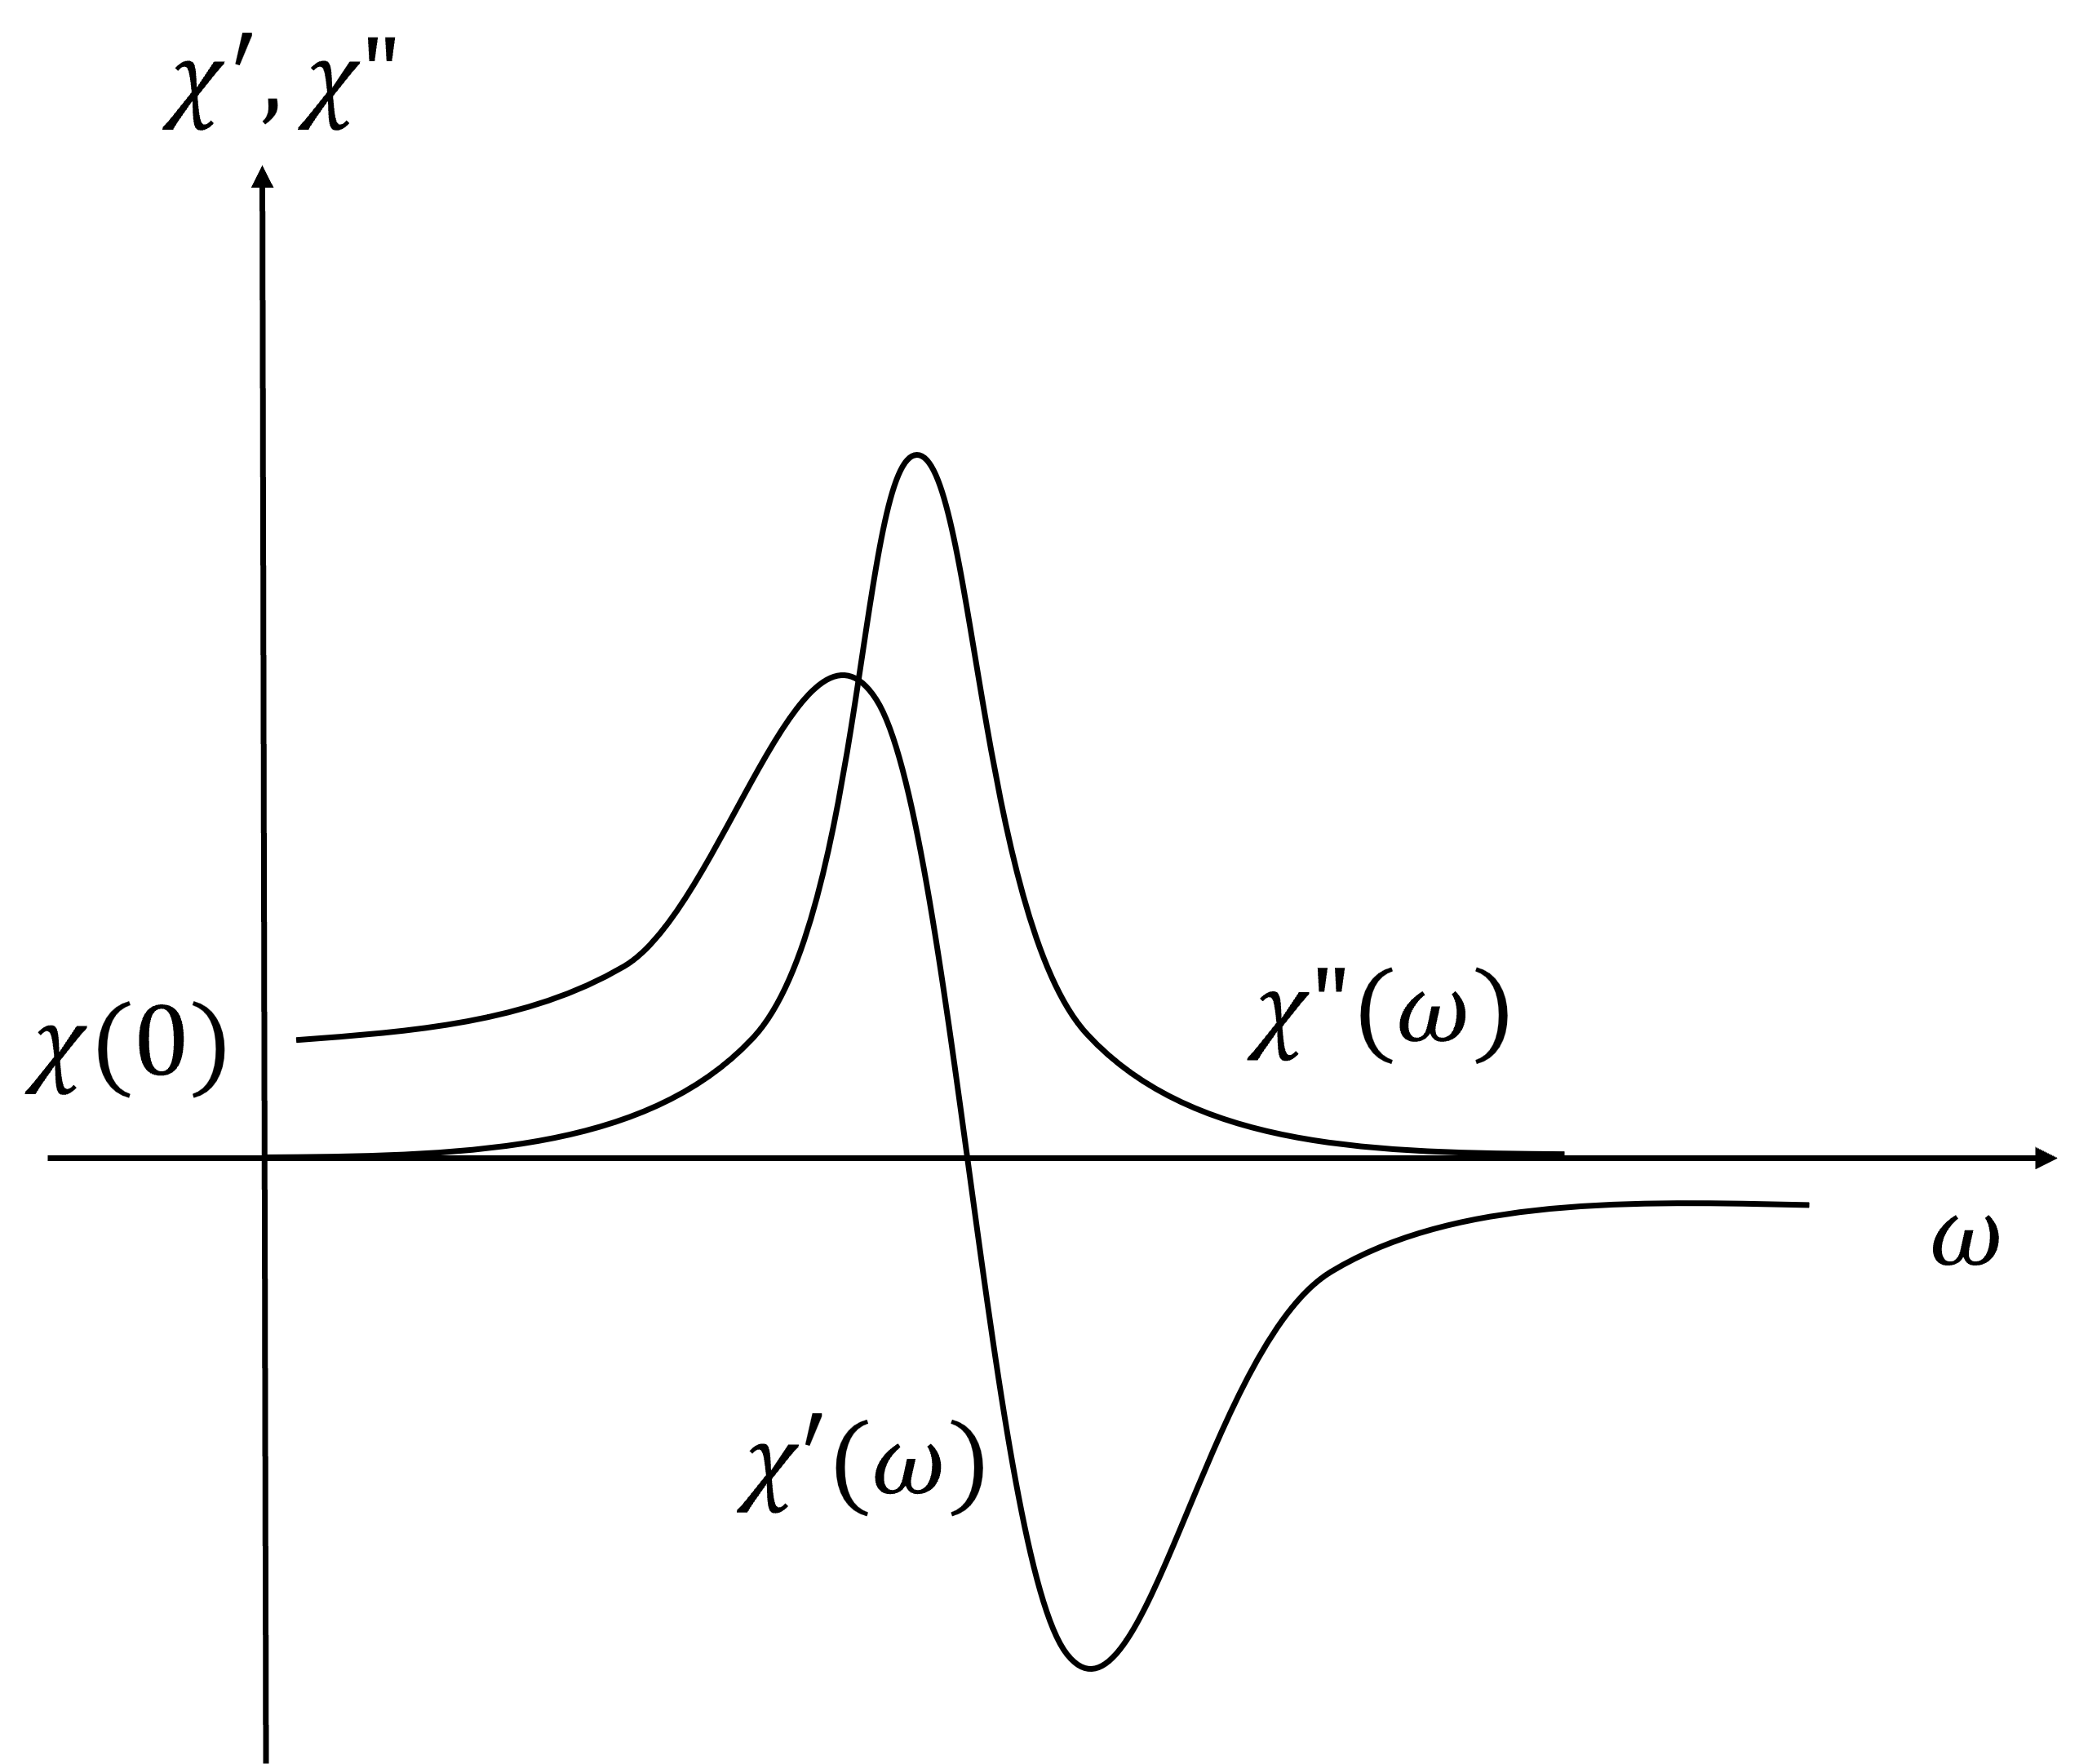
\includegraphics[width=100mm]{./figure/outou.png}
  \caption{磁化率の実部、虚部の周波数依存性}
  \label{outou}
\end{figure}



\chapter{先行研究}

\section{Tsai型近似結晶の磁性}
2021年東京理科大学の鈴木氏らは、Tsai型準結晶近似体の磁性に関する包括的な調査を行い、特に1/1および2/1近似体の磁気的性質について詳述している。
本研究の主な焦点は、希土類元素(R)を含むTsai型1/1近似体において、電子数(e/a比)が磁気秩序に与える影響である。e/a比は準結晶やその近似体の磁気挙動を制御する重要なパラメータであり、特に磁化のCurie-Weiss温度($\theta_p$)や磁気秩序がe/a比に応じて系統的に変化することが示された。\par
Tsai型近似体の磁化率測定では、異なるe/a比に対応して強磁性(FM)、反強磁性(AF)、およびスピングラス的な状態が観察された。特に、反強磁性状態では磁化率が低温で尖ったピークを示し、反強磁性転移温度($T_N$)が特定され、スピンフロップ現象が低磁場で見られたことから、異なる磁気秩序が存在することが示唆された。さらに、e/a比が1.54から2.16の範囲で、AF、FM、スピングラスの各領域が交互に出現することが観察され、特に反強磁性領域がTb系で広がっていることが示唆されている。スピン系における異方性が磁気秩序の形成に重要な役割を果たしていることも示唆された。よって、1/1近似体の磁気相図が2/1近似体にも適用できる可能性が明らかになった。磁化率測定の結果からも、Tsai型準結晶近似体の磁気相が電子数に依存して変化することが確認され、今後の準結晶やその近似体における未発見の磁気相の探索に向けた基盤が提供された。



\begin{figure}[htbp]
  \centering
  \vspace{10mm}
  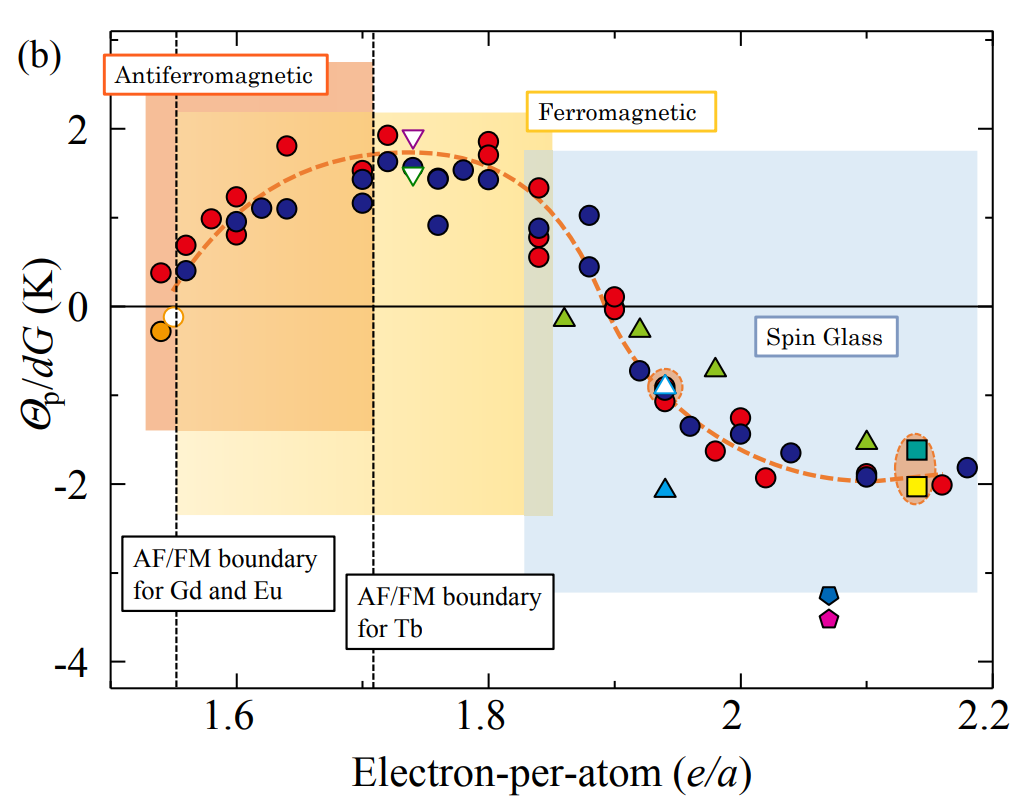
\includegraphics[width=100mm]{./figure/e_a.png}
  \caption{磁性の周期関数的変化}
  \label{e_a}
\end{figure}
\begin{figure}[htbp]
  \centering
  \vspace{10mm}
  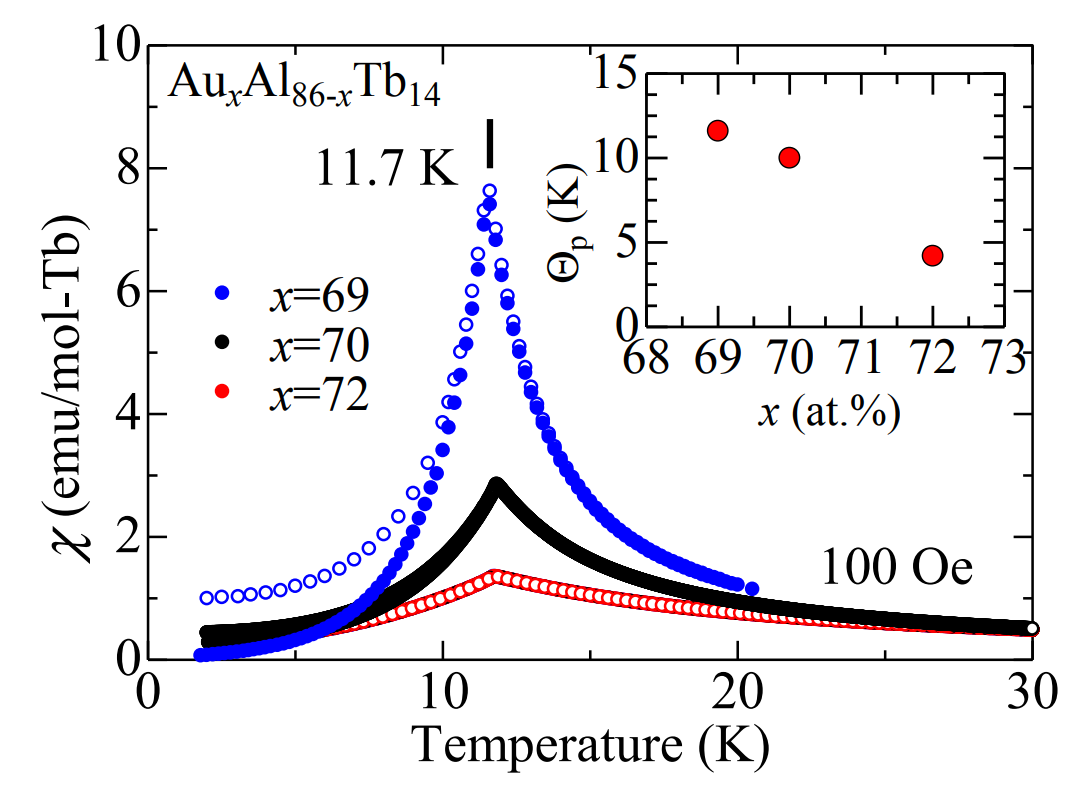
\includegraphics[width=100mm]{./figure/qi.png}
  \caption{磁性の周期関数的変化}
  \label{χ}
\end{figure}

\section{近似結晶における渦巻スピン秩序}

\chapter{提案手法}
\section{---}
\subsection{---}
\subsection{---}
\section{---}
\subsection{---}
\subsection{---}

\chapter{評価実験}
\section{実験方法}
\section{実験結果}
\section{考察}

\chapter{まとめ}
研究のまとめ。なんやかんやなんやかんやなんやかんやなんやかんやなんやかんやなんやかんやなんやかんやなんやかんやなんやかんやなんやかんやなんやかんやなんやかんやなんやかんやなんやかんやなんやかんやなんやかんやなんやかんやなんやかんやなんやかんやなんやかんや
なんあやかあjaaaaaaaaaaaa
%=====================================================================================
\chapter*{謝辞} %章を付けずにタイトル表示
\addcontentsline{toc}{chapter}{謝辞} %章立てせずに目次に追加するおまじない
本論文を作成するにあたり、---- みなさまに感謝の意を表します.aaaaaaaa

%=====================================================================================

\addcontentsline{toc}{chapter}{参考文献} %章立てせずに目次に追加するおまじない
\renewcommand{\bibname}{参考文献} %これがないと,タイトルが「関連図書」になってしまう
\bibliography{bibtexファイル名} %bibtexファイルの読み込み
\bibliographystyle{junsrt} %本文に\cite{}を入れることで,参考文献表示

\end{document}

